% Pages in Thesis should have one of standard U.S. Paper Sizes
% U.S Letter Paper (8.5 x 11) is used.
% Body should be either 11 pt or 12 pt type.
\documentclass[12pt, letterpaper]{thesis}

\usepackage{hyperref}
\usepackage[sorting=debug]{biblatex}
\usepackage{afterpage}
\addbibresource{references.bib}
% For mathematical symbols such as degree
\usepackage{textcomp}
\usepackage{gensymb}
\usepackage{booktabs}

\date{}
\begin{document}

% Front Matter
% Except for the "Abstract" page, every page of thesis must be assigned a
% page number. Placement of consistent page numbers is necessary, and they
% must either be at center, or at the top-right corner.
% Page numbering should be roman numerals for the front matter, and numbered
% for main text.
% Hide page numbers for this page.
\thispagestyle{empty}
\begin{center}
    LOREM IPSUM TITLE LOREM IPSUM
    
    by
    
    AASHISH YADAVALLY
    
    (Under the Direction of Frederick Maier)
    
    ABSTRACT
\end{center}

Lorem ipsum dolor sit amet, consectetur adipiscing elit, sed do eiusmod tempor incididunt ut labore et dolore magna aliqua. Ut enim ad minim veniam, quis nostrud exercitation ullamco laboris nisi ut aliquip ex ea commodo consequat. Duis aute irure dolor in reprehenderit in voluptate velit esse cillum dolore eu fugiat nulla pariatur. Excepteur sint occaecat cupidatat non proident, sunt in culpa qui officia deserunt mollit anim id est laborum.

\vspace{\baselineskip}
\noindent
INDEX WORDS: Lorem Ipsum

\newpage
\pagenumbering{roman}
% Hide page numbers for this page.
\thispagestyle{empty}

\begin{center}
    LOREM IPSUM TITLE LOREM IPSUM
    
    \vspace*{2\baselineskip}
    by

    \vspace*{2\baselineskip}
    AASHISH YADAVALLY
    
    B.Tech., Indian Institute of Information Technology Vadodara, INDIA, 2018
    \vspace*{4\baselineskip}

    A Thesis Submitted to the Graduate Faculty of The University of Georgia
    in Partial Fulfillment of the Requirements for the Degree
    \vspace*{3\baselineskip}

    MASTER OF SCIENCE
    \vspace*{3\baselineskip}

    ATHENS, GEORGIA
    
    2020
\end{center}

\newpage
% Hide page numbers for this page.
\thispagestyle{empty}

\begin{center}
    \vspace*{18\baselineskip}
    \textcopyright \hspace{0.05cm} 2020
    
    Aashish Yadavally
    
    All Rights Reserved
\end{center}

\newpage
% Hide page numbers for this page.
\thispagestyle{empty}
\newgeometry{top=1.75in, left=1.5in, right=1in, bottom=1in}

\begin{center}
    LOREM IPSUM TITLE LOREM IPSUM
    
    \vspace*{1\baselineskip}
    by
    \vspace*{1\baselineskip}

    <INSERT-NAME-HERE>
\end{center}

\vspace*{8\baselineskip}

\begin{flushright}
Major Professor: $\hskip 0.5em$ <INSERT-ADVISOR-NAME-HERE>
\vspace{\baselineskip}

Committee: $\hskip 2.25em$ <INSERT-NAME-HERE> $\hskip 0.05em$ \\
<INSERT-NAME-HERE> $\hskip 3.3em$
\end{flushright}

\vspace{4\baselineskip}
\noindent
Electronic Version Approved:\\
Suzanne Barbour\\
Dean of the Graduate School\\
The University of Georgia\\
May 2020
\newpage

\chapter{1}{Acknowledgements}{Acknowledgements}
\par I would like to thank all my committee members for their time and the numerous suggestions they provided throughout my research. In particular, I would like to thank Dr. Maier for his guidance, constant encouragement and motivation to keep me going. I owe a great debt to Zachary Jones and Chris Barrick who facilitated my introduction into the project, and whose contributions to the project laid the foundation for my work. I am thankful to my friends and family who kept me sane during these unprecedented times, where the whole world has come to a standstill due to COVID-19. I would like to thank everyone at the \textit{Institute for Artificial Intelligence} who presented me with the opportunity to be a part of this project, and also Ms. Tino, who made my life easier by helping me with the mundane administrative tasks.

\newpage
\listofchapter
\newpage
\listoftables
\addcontentsline{chl}{chapter}{~LIST OF TABLES}
\newpage
\listoffigures
\addcontentsline{chl}{chapter}{~LIST OF FIGURES}
\newpage

% Chapters in Thesis
% Chapter 1: Introduction
\pagenumbering{arabic}
\chapter{}{Introduction}{Introduction}
\par Climate change is widely considered to be a major environmental crisis that we face today. Transitioning from fossil fuel based energy sources to renewable energy sources is one of the most powerful ways in which we can reduce our ecological footprint as a society. However, owing to the unpredictability associated with carbon-free sources such as solar energy and wind energy, incorporating them into an electrical energy structure is challenging. The unpredictable nature of solar radiation also leads to a number of other problems such as voltage fluctuations, stability issues, etc. Thus, to ensure a balance between the consumption and production of solar energy, accurate prediction of solar irradiance is of utmost importance, as this is a measure of the available fuel of a solar power generator at a given future moment in time. \cite{exec_summary_1}

\par Solar irradiance forecasting can be performed by several methods depending on the temporal variability of the forecast horizon, ranging from a minute to several days. However, the predictions worsen as the forecast horizon increases. Numerical weather prediction (NWP) models use mathematical models of atmosphere and oceans to predict weather variables up to two days and beyond. Thus, using such physical weather forecast models for day-ahead solar forecasting is a common strategy. National Oceanic and Atmospheric Administration (NOAA) maintains various global and mesoscale weather prediction models for weather forecasting. Mesoscale models are three-dimensional regional models based on thermodynamic equations describing the physical processes. They are efficient in predicting smaller scale detail. North America Mesoscale (NAM) Forecast System \cite{litrev_nwp_nam} is one of the major mesoscale-based weather forecast models maintained by NOAA.

\par The purpose of this work is to effectively predict surface-level solar irradiance 24 hours into the future, at different fixed and tracking solar arrays located at a solar farm near the University of Georgia. Towards accomplishing this, NAM weather forecasts were used for solar irradiance forecasting, which is an integral part of this work. The NAM Forecast System releases four forecasts in a day at six-hour intervals (00h, 06h, 12h, 18h UTC) for multiple $12km$ x $12km$ grids spanning \restoregeometry\noindent the continental United States. NAM data for the years 2017 and 2018 were collected and analyzed.

\par Among the different weather variables modeled by NAM Forecast System, downward short-wave radiation flux parameter (synonymous with global horizontal irradiance, GHI \cite{multimodel_overpredict}), which is an estimate of the total amount of short-wave radiation (radiation with wavelength between $0.2\mu m$ and $3.0 \mu m$) that reaches the Earth's surface, is essential for short-term solar forecasting. Thus, GHI was post-processed with respect to the surface-level solar irradiance using multiple machine learning models. Furthermore, site-specific information was incorporated into the models by including additional weather variables such as surface temperature, total cloud cover and atmospheric height. However, one major drawback in this setup was that the GHI measured by the NAM Forecast System is  variable, depending on the cloud conditions. Thus, the need to empirically correct the bias in this parameter was identified and techniques in this regard were explored.

\par The radiation from the sun reaching the earth surface is a combination of direct normal irradiance (DNI) and diffused horizontal irradiance (DHI), which together amount to the global horizontal irradiance (GHI). Of the global solar radiation reaching the earth's surface, DNI is the direct radiance received on a plane perpendicular to the earth's surface. DHI is the fraction of global solar radiation scattered by particles in the atmosphere. GHI, in turn, is the fraction of global solar radiation reaching the earth's surface on a plane horizontal to the surface. Several formulations have been proposed to estimate these metrics from environmental conditions. Of these, the \textit{Clear-sky Scaling} technique \cite{pvlib_ineichen} and \textit{Liu-Jordan} \cite{pvlib_liujordan2} method were studied. The irradiance metrics retrieved through these formulations were used to correct the bias in the GHI estimate from NAM Forecast System. 

\par This thesis documents various experiments we conducted towards improving the efficacy of solar irradiance prediction, and can be divided into four chapters (1 through 4) in this fashion: Chapter 1 discusses the problem formulation and motivation for the approach we undertook to forecast solar irradiance. In Chapter 2, several research works were reviewed which discuss the methodologies undertaken by various solar forecasting researchers depending on the forecast horizon of the predictions or the spatial resolution of the input data. Major empirical solar radiation models which formulate the irradiance metrics described above, and which can be broadly classified into \textit{decomposition models} and \textit{parametric models} are briefly discussed. Furthermore, recent works undertaken at the University of Georgia, related to solar irradiance forecasting are reviewed, as this lays a basis to build upon and compare the results obtained in this work.

\par Jones et al. \cite{thesis_zach} developed a machine learning pipeline to forecast day-ahead solar irradiance using the weather forecast data from the NAM Forecast System. Chapter 2 begins by replicating the results obtained in \cite{thesis_zach}, which used nine weather variables from the NAM data. However, they did not include the \textit{total cloud cover} parameter, which is defined as the fraction of the sky covered by visible clouds. Cloudiness is considered to be one of the most important meteorological factors determining the amount of solar radiation reaching the earth surface. Thus, all the ten features were further analyzed with respect to the target irradiance observations recorded at the solar farm, intending to quantify their usefulness in the day-ahead irradiance prediction. It was identified that weather variables such as surface temperature, global horizontal irradiance, total cloud cover and atmospheric height were more significant. 

\par Each of the weather variables in the NAM data has 36 feature projections at a 1-hour temporal resolution, and the remaining at a 3-hour temporal resolution. Jones et al. \cite{thesis_zach} used all 36 feature projections at 1-hour temporal resolution for the nine weather variables as predictors for machine learning models. To rationalize this scheme, 24 feature projections of the GHI weather variable were compared with irradiance observations from the fixed solar array for all 24 target hours in the forecast horizon. It was observed that the target irradiance observations for a particular target hour did not depend on all the feature projections of the weather variable. Thus, 13 feature projections (from 6 hours prior to the target hour to 6 hours ahead of the target hour) of all weather variables were chosen as predictors for each of the target hours in the forecast horizon separately. This input-selection scheme helped in reducing the computational cost of training the machine learning models significantly. In one series of experiments, results obtained through this scheme were compared with those obtained by replicating the methodology followed in \cite{thesis_zach}. An average improvement in performance (across different machine learning models) by \_\_\_ was recorded, with the best machine learning model having a mean absolute error (MAE) of $\_\_ W/m^2$, $\_\_ W/m^2$, $\_\_ W/m^2$ for the dual-axis tracking solar array, fixed-axis solar array and single-axis tracking solar array respectively.

\par Another series of experiments were performed to test the effect of the geographic expansion of forecast coverage by including additional weather forecasts from area surrounding the target location. In \cite{thesis_zach}, Jones et al. included weather forecasts from a grid of cells surrounding the NAM data grid representing Athens. They noted that considering a $3 x 3$ grid of cells was most appropriate towards the solar irradiance prediction, and that the geographic expansion had diminishing returns for grid sizes greater than $3 x 3$. However in this work, it was observed that such a geographic expansion following the input selection scheme described earlier did not help in improving the solar irradiance predictions, and the $1 x 1$ grid, i.e. just considering the NAM data grid representing Athens was more appropriate. In fact, in a few cases, the geographic expansion also had a detrimental effect in performance.

\par Furthermore, the analysis of the machine learning models was extended in two ways: a stratified analysis for each of the forecast hours was performed, wherein the ability of the models to predict the diurnal aspects of the forecasts was gauged; a seasonal analysis was performed, wherein the ability of the models to realize the seasonal characteristics was gauged. Considering the target location is in Georgia, United States, which experiences four major seasons i.e. \textit{spring}, \textit{summer}, \textit{autumn} and \textit{winter}, the seasonal analysis was performed for each of these seasons exclusively. 

\par In Chapter 4, a multi-model blending approach is introduced to address the bias in GHI recorded by NAM Forecast System. In this approach, the GHI recorded by NAM Forecast System is combined with GHI formulated with the help of empirical solar radiation models such as \textit{Clear-sky Scaling} and \textit{Liu-Jordan Model} based on metrics such as clear-sky index ($k_c$) and clearness index ($k_t$). The clear-sky index can be defined as the ratio of measured GHI ($GHI_{NAM}$) to GHI in clear-sky conditions ($GHI_{CS}$), estimated through the \textit{clear-sky scaling} technique. This measure was estimated by truncating the ratio to values between 0 and 2, 0 indicating overcast conditions and 2 indicating a clear day, i.e. sky conditions defined by the absence of visible clouds. It was observed that there was a high variability in this parameter for only the 18h NAM forecasts from among the 00h, 06h, 12h and 18h forecasts released by the NAM Forecast System. Thus for all 18h forecasts with $k_c > 1.5$, $GHI_{NAM}$ and $GHI_{CS}$ were averaged. This resulted in an average improvement in performance (across different machine learning models) by \_\_\_\_\_, the best performing model having a mean absolute error (MAE) of $\_\_ W/m^2$, $\_\_ W/m^2$, $\_\_ W/m^2$ for the dual-axis tracking solar array, fixed-axis solar array and single-axis tracking solar array respectively.

\par A similar model blending approach was carried out between the \textit{Liu-Jordan} model and the NAM Forecast System based on the \textit{clearness index} metric. Clearness index is a measure of the clearness in atmosphere, and can be defined as the ratio between the solar radiation transmitted through the atmosphere to the solar radiation reaching the earth's surface. The clearness index measure is critical in the formulation of irradiance metrics using \textit{Liu-Jordan} model, and thus, using it to contrast the GHI recorded by NAM Forecast System and Liu-Jordan model is intuitive. Thus for all 12h and 18h forecasts, for which GHI is significant, $k_t$ was estimated. In order to gauge the variability of the clearness index better, it was truncated to values between 0 (overcast conditions) and 2 (clear atmosphere). For the forecasts with $k_t > 0.7$, $GHI_{NAM}$ and $GHI_{LJ}$ were averaged. DHI estimated by the \textit{Liu-Jordan} model was identified to be an important parameter in solar irradiance predictions as well. Thus, it was included along with the weather parameters from the NAM Forecast System as predictors for the different machine learning models. This methodology resulted in an average improvement in performance (across different machine learning models) by \_\_\_\_\_, the best performing model having a mean absolute error (MAE) of $\_\_ W/m^2$, $\_\_ W/m^2$, $\_\_ W/m^2$ for the dual-axis tracking solar array, fixed-axis solar array and single-axis tracking solar array respectively.

\newpage
% Chapter 2: Related Work
\chapter{}{Literature Review}{Literature Review}
\par High variability in solar radiation necessarily results in variability in the output of photovoltaic (PV) power plants. What this essentially means is that, in order to effectively integrate PV systems into a larger electrical grid (which must compensate for the variable output of PV systems to ensure overall stability), effective prediction of solar irradiance is needed. In the last few decades, solar forecasting researchers have developed a variety of data-driven approaches to improve solar irradiance forecasting. Most of these approaches can be categorized based on the resolution of the forecast horizon, ranging from a few minutes to a couple of days, weeks or months; and the spatial resolution of the input data pertaining to a particular location. 

\par For solar irradiance forecasts up to $<30$ minutes ahead, a variety of techniques based on the ground-to-sky imagers have been explored. The spatial resolution for the total sky imagery is in the range of 10m - 100m. Using the sky images taken every 30 seconds, Chow et al \cite{litrev_intrahour1} presented a method for determining sky cover and solar irradiance nowcasting. Marquez et al. \cite{litrev_intrahour2} used image-processing techniques to calculate velocity fields and classify clouds in individual grids so as to employ it to forecast Direct Normal Irradiance (DNI), an essential component of global irradiance, for time horizons ranging from 3 minutes to 15 minutes.

\par Statistical time-series models such as Auto Regressive Integrated Moving Average (ARIMA) and non-linear model approximators such as Artificial Neural Networks (ANNs) have been shown to be more effective for forecasting solar irradiance up to $2$ hours ahead \cite{litrev_ts1}. Marquez and Coimbra \cite{litrev_ts2} successfully used meteorological variables from US National Weather Service (NWS) Forecasting database as inputs to an ANN model for forecasting global and direct solar irradiance. In \cite{litrev_ts3}, Reikard reviewed a variety of time-series modeling techniques for predicting solar irradiance, and observed that the ARIMA models, in general, had the best forecasting results. However, as Lopez et al. \cite{litrev_ts4} note, these developed models are not transferable to different locations, especially ones with varying cloudiness properties (this certainly applies to the work at UGA as well).

\restoregeometry

\par Input data from satellite imagery tracking cloud motion has been shown to be useful for an \textit{intra-day} forecast horizon between 1 hour and 24 hours. The geostationary satellites detect clouds with the help of visible and infra-red images, which generally have a spatial resolution of $\sim$1 km. Various methods such as Heliosat-I \cite{litrev_sat1}, Heliosat-II \cite{litrev_sat2} and Heliosat-III \cite{litrev_sat3} have been implemented which employ motion-vector fields to track the clouds using these images. By applying the calculated motion vector fields on the actual image, the cloud index images can be determined. Hammer et al. \cite{litrev_sat4} employed Heliosat-I technique on such cloud index images for forecasting solar irradiance $\sim$30 minutes to 6 hours in future. Cloudiness has a significant impact on the surface solar irradiance, and the basis of this methodology relies upon the determination of cloud structures.

\par For a \textit{days-ahead} solar forecasting range which is essential for utility applications, the knowledge of the meteorological weather parameters in that period is paramount. Numerical Weather Prediction (NWP) models are physical models which make use of the current meteorological conditions and predict weather conditions days into the future, on the basis of atmospheric equations. Notably, NWP models are able to forecast up to two days ahead or beyond, depending on the spatial domain of the model. Examples of the NWP models maintained by the National Oceanic and Atmospheric Administration (NOAA), which record data across different spatial resolutions, across varying geographical expanse are the Global Forecast System (GFS) \cite{litrev_nwp_gfs}, North American Mesoscale (NAM) \cite{litrev_nwp_nam}, Rapid Refresh (RAP) and High Resolution Rapid Refresh (HRRR).

\par Several researchers have concentrated their efforts on comparing the effectiveness of each of the NWP models for solar irradiance forecasting purposes at various locations. Mathiesen and Kleissl \cite{litrev_nwp1} compared the irradiance parameter forecast in NWP models such as NAM, GFS and ECMWF within the continental United States, with respect to solar forecasting. In this work, they extensively studied the predictions using each of the NWP models in varying cloud conditions, establishing a database to validate numerical weather predictions. In \cite{litrev_nwp2}, Ruiz-Arias et al. found that the NWP models based solar irradiance forecasting \textit{significantly outperforms} satellite-based methodologies while forecasting 6 hours and beyond, and attributed it to the effective simulation of weather parameters of the entire atmospheric system in the NWP models.

\par Lorenz et al. \cite{litrev_nwp3} performed benchmarking studies to gauge the reliability of different solar irradiance forecasting approaches. They investigated the seasonal dependence of forecast errors using several techniques. They concluded that post-processing the weather parameters in the NWP models significantly captures the dependence between forecast accuracy and climatic conditions. Perez et al. \cite{litrev_nwp4} validated the performance of the NWP models across seven stations in the SURFRAD network. They extracted the hourly GHI forecasts by time-interpolating the 3-hour and 6-hour cloud cover parameter forecasts in the NWP models, and further adjusting them using sky-cover-to-irradiance fits. In this work, the authors explored a diverse set of climatic environments and noted that the models' performance in winters tends to be poorer than in summers. They also concluded that forecasts from the one-hour time-interpolated data are on par or better than the forecasts from the satellite-imagery based data for a forecast horizon up to 5 hours.

\par In \cite{litrev_nwp1}, Mathiesan and Kleissl also infer that the NWP models like GFS and NAM are biased towards forecasting clear conditions resulting in large biases in global horizontal irradiance (GHI) parameter in these conditions. They obtain the metric Mean Bias Error (MBE) for each NWP model based on the solar zenith angle and the clear sky index ($k_c$) metric, which is the ratio of the measured GHI in the model to the clear sky GHI. However, like Diagne et al. \cite{litrev_nwp5} note, the methodology used by Mathiesan and Kliessl was not adequate, as they did not present information about the bias source, which is important to selectively correct forecasts. They observed that these bias corrections did not help in reducing the Root Mean Squared Error (RMSE) metric, as even the accurate forecasts were unnecessarily corrected - indicating a need for a better approach for GHI bias corrections in the NWP models.

\par The effectiveness of physical NWP models such as the NAM Forecast System for the purpose of day-ahead solar irradiance forecasting, demonstrated in the aforementioned works, prompted us to study and analyze it further. Accurate identification of clear-sky conditions is essential towards selectively correcting the bias in GHI \cite{litrev_nwp6}. Such an identification requires additional measurements such as direct or diffuse components of global solar irradiance, which is not measured by the NAM Forecast System. However, these irradiance components can be estimated by means of empirical solar radiation models. The main difference between physical models such as the NAM Forecast System and empirical solar radiation models is that the former parameterizes cloud microphysics through mathematical equations, while the latter formulates the relation between meteorological variables derived through experimental observations. 

\subsubsection*{Empirical Solar Radiation Models}
\par  Several empirical formulations have been proposed in literature which help predict the irradiance metrics such as global horizontal irradiance (GHI), diffuse horizontal irradiance (DHI) and direct normal irradiance (DNI) from atmospheric properties. GHI is the total amount of shortwave radiation reaching a surface horizontal to the ground, and is the most useful solar radiation data parameter. In comparison, DHI is the part of global solar radiation which passes through the atmosphere, and is absorbed, scattered or reflected by the gases in the atmosphere. DNI is the amount of solar radiation received by a surface that is held normal to the rays from the sun. It needs emphasis because of the sharp shadows that it can extend on the surface of the earth. Irradiance on the surface of a solar cell can be determined with the help of DNI, and thus, proper estimation of DNI is of high importance in Concentrated Solar Power (CSP) systems \cite{litrev_pvlib2}.

%DHI needs emphasis because of the sharp shadows that it can extend on the surface of the earth \cite{litrev_pvlib1}.

\par The empirical solar radiation models to estimate the sky (DHI) and beam (DNI) components of global solar radiation can be categorized into \textit{parametric} and \textit{decomposition} models \cite{litrev_pvlib3}. Parametric models require detailed information about atmospheric conditions such as turbidity, cloud cover, precipitable water content, etc. to be able to calculate DHI and DNI. In comparison, the decomposition models formulate empirical equations to estimate DHI and DNI from GHI, based on the correlations between each of the components. The parametric models are a better alternative to decomposition models only in cases where the meteorological data is not available \cite{litrev_pvlib3}\cite{litrev_pvlib4}.

\par Radiative Transfer Models (RTMs) help in simulating the radiative transfer of electromagnetic radiation through a planetary atmosphere, and thus help in estimating solar irradiance. However, they are computationally expensive to maintain. The clear-sky solar irradiance parametric models provide relatively simple parameterizations to estimate solar irradiance in conditions with less visible clouds \cite{litrev_pvlib8}. The aerosols and water vapour present in the atmosphere play a significant role in scattering the sunlight, and have an impact on the amount of solar radiation reaching the Earth's surface. Thus, solar forecasting researchers concentrated their efforts towards estimating GHI in clear-sky conditions, i.e, conditions where visible clouds are negligible, and further scaling this parameter across cloud conditions. 

\par Bird and Hulstrom \cite{litrev_pvlib9} proposed the \textit{Bird Clear Sky Model} based on comparisons of results from the radiative transfer codes, to estimate clear sky direct beam, hemispherical diffuse, and total hemispherical solar radiation on a horizontal surface. However, one of the drawbacks with this model is that various atmospheric parameters such as aerosol optical depth, ozone and water vapour are fixed for an entire year. Gueymard \cite{litrev_pvlib10} proposed the \textit{REST2 Clear Sky Model} which specifically accounts the effects of aerosols to predict cloudless-sky broadband irradiance. The REST2 model represents broadband components of two different spectra, and incorporates the transmission estimates for each of the spectra separately. Finally, the total diffuse radiation on a horizontal surface is aggregated from the estimates of both the spectra.

\par \textit{Ineichen and Perez} \cite{litrev_pvlib14} proposed a new airmass independent formulation to estimate the Linke Turbidity coefficient, thus removing it's dependency on solar geometry, and used the coefficient to develop two clear-sky models to estimate global and direct normal irradiance. Furthermore, Ineichen \cite{litrev_pvlib11} modified the original version of the \textit{Solis Clear Sky Model} proposed by Mueller et al \cite{litrev_pvlib12} to accommodate the circumstances in which spectral computations aren't possible, by introducing a broadband version of the algorithm. 

\par The decomposition models are formulated on the basis of the \textit{clearness index} ($k_t$) parameter, which is the ratio of the measured solar radiation to the extraterrestrial solar radiation. A higher value ($k_t \rightarrow 1$) of the clearness index parameter indicates that the atmosphere is clear, while a lower value ($k_t \rightarrow 0$) of the clearness index parameter indicates that the atmosphere is cloudy. Chandrasekaran and Kumar \cite{litrev_pvlib5} collected data in Madras, India to formulate a fourth-order polynomial correlation depending on the clearness index parameter to estimate the irradiance metrics in a tropical setting \cite{litrev_pvlib6}.

\par By analyzing the data collected across multiple locations in the United States and Canada, \textit{Liu and Jordan} \cite{litrev_pvlib7} formulated an empirical equation on the basis of the clearness index parameter to estimate the irradiance metrics. Maleki et al \cite{litrev_pvlib3} reviewed various solar radiation models, and observed that the Liu and Jordan model is very effective in estimating diffuse radiation on inclined surfaces.

\subsubsection*{Recent Work on Solar Irradiance Forecasting at the University of Georgia}
\par "Georgia Power", a regional utility company, recently partnered with the University of Georgia (UGA) to set up a 1MW solar facility in Athens, GA. The facility consists of multiple fixed and tracking (single-axis and dual-axis) solar arrays. Recent work at UGA has been devoted to analyzing or predicting solar radiation based upon the data provided by the facility and the GAEMN (Georgia Automated Environmental Monitoring Network) weather station network.

\par In \cite{publication_sanders}, Sanders investigated the importance of different weather variable observations in the prediction of solar irradiance. From among the sixteen weather variables recorded by GAEMN, he obtained current and historical weather information for the following weather variables which are typically known to affect solar irradiance: air temperature, precipitation rate, visibility, wind speed, wind direction, dew point temperature, air pressure and relative humidity. Utilizing the solar radiation data from GAEMN, they built predictive models including current weather observations, weather forecasts from NWP models for the target location, and additional weather forecasts from NWP models for area surrounding the target location. 

\par In addition, they obtained NWP model predictions for these weather variables at the target locations to analyze the effect of using NWP model predictions for these variables as a means of forecasting solar radiation over one-hour and 24-hour time frames. Upon including the weather forecast data in the predictive models, it was observed that there was a reduction in mean absolute error (MAE) for 1-hour predictions by 7.6\% and for 24-hour predictions 40.2\%. They noted that the incorporation of weather forecasts from NWP Forecast System is extremely important in solar forecasting, especially over a longer time horizon. 

\par Sanders \cite{publication_sanders} performed work based on Lorenz et al. \cite{expansion_lorenz}, who found that expanding the forecast region to approximately $100 km$ x $100km$ and performing a spatial averaging across the region resulted in an improvement in day-ahead solar forecasting. Larson et al. \cite{pvlib_larson} noted that the solar radiation predictive models which use NWP data can usually be improved by averaging the GHI forecasts from NWP grid points surrounding the target location. Sanders \cite{publication_sanders} validated these findings by including weather forecasts from areas surrounding the target location, and found that it was extremely beneficial, especially while forecasting over a longer time horizon, where the weather system is less predictable. This was performed by including forecasted weather variables from the NWP cells lying to the north-west, north, north-east, east, south-east, south, south-west and south, resulting in eight additional parameters for each weather variable. They found that such a methodology led to an increase in predictive accuracy in both one-hour ad 24-hour solar radiation predictions.

\par Jones \cite{thesis_zach} extended the work in \cite{publication_sanders} by developing machine learning models for hourly targets from 1 - 24 hours, using GAEMN observational data and NWP predictions (Rapid Refresh, RAP and North American Mesoscale, NAM). He observed that the forecasted weather variables from NWP models became more important for target hours beyond a very short forecast horizon. In addition, utilizing the solar irradiance observations from the solar farm, they presented a case-study in irradiance prediction by augmenting these observations along with the NAM data. They explored the geographic expansion of forecast coverage by including the NAM weather forecasts from a grid of cells around the NAM data grid representing Athens, towards obtaining a $3$ x $3$ geographical grid shape, representing a geographical expanse of $36km$ x $36km$. It was observed that using the $3$ x $3$ grid shape was optimal for solar irradiance forecasting at the farm, and it improved the accuracy significantly as compared to just considering weather forecasts from the NAM data grid representing Athens. Using the $3$ x $3$ grid shape, they achieved the best accuracy with an MAE of $47.6$ $W/m^{2}$ for the fixed-axis solar array, $58.7$ $W/m^{2}$ for single-axis tracking solar array and $75.4$ $W/m^{2}$ for dual-axis tracking solar arrays.

\par Jones \cite{thesis_zach} attempted to quantify the improvement in accuracy of predictive irradiance models as a result of the expansion of forecast coverage. Two of the best-performing machine learning models for the $3$ x $3$ grid shape, \textit{k-Nearest Neighbors} and \textit{Random Forests} were retrained for $5$ x $5$ and $7$ x $7$ grid shapes as well, representing a geographical expanse of $60km$ x $60km$ and $84km$ x $84km$ respectively, and their performance in $MAE$ and $R^2$ were recorded. They realized that the benefits from a wider geographic coverage of forecasted weather variables resulted in diminishing returns as the size grows larger. While the improvement due to using $3$ x $3$ grid shape over $1$ x $1$ grid shape (representing Athens) was significant (\textasciitilde 16\%), those for $5$ x $5$ and $7$ x $7$ grid shapes over $3$ x $3$ was negligible.
\newpage
% Chapter 3: Multi-model Solar Irradiance Forecasting
\chapter{}{Multi-Model Approach to Solar Irradiance Forecasting}

\subchapter{Overview}
For days-ahead forecast horizon, regional and global numerical weather prediction models, predicting the evolution of the atmospheric system have been shown to be more appropriate and accurate \cite{thesis_zach}. The numerical weather prediction models derive their initial conditions from different ground and airborne sensors from across the world. Based on thermodynamic equations describing the physical processes occurring in atmosphere, they forecast different weather variables into the forecast horizon. The National Oceanic and Atmospheric Administration (NOAA) operates a variety of numerical weather prediction models with their spatial resolution ranging from approximately 10 km - 50 km, and their temporal resolution typically being 1 hour or 3 hours -  which are normally updated every 6 hours \cite{multimodel_bestpractices}. 

\par In this work, we intended to forecast solar irradiance captured at the solar farm in Athens, Georgia for a forecast horizon of 24 hours. For this purpose, a mesoscale model such as the \textit{North American Mesoscale (NAM)} Forecast System \cite{multimodel_nam} which can predict parameters describing cloudiness was used. Typical weather variables known to affect solar irradiance forecasting systems such as air temperature, geopotential height, cloud cover, visibility, wind speed, dew point temperature, air pressure, downwelling shortwave radiation flux, downwelling longwave radiation flux, and humidity were evaluated so as to gauge their effect on the solar irradiance predictions. It was observed that the irradiance readings from the solar farm for each of the arrays were influenced more by the surface temperature, downwelling short-wave radiation flux, total cloud cover, and atmospheric height. Thus, the remaining weather variables were discarded. This enabled a cut in computational cost of modeling and also led to an improvement in the performance of the models.

\restoregeometry

\par Downwelling shortwave radiation flux, synonymous with global horizontal irradiance (GHI) is measured by NWP models using columnar radiative transfer models (RTM). The RTMs help in determining cloud optical properties for different wavelength bands with the help of weather variables such as air temperature, gas concentrations and cloud structure. Thus, they contribute to effective cloud modeling, and in turn, effective shortwave radiation flux computation. However, the direct output from the mesoscale models has shown severe deviations between forecasted and real irradiance \cite{multimodel_ghi}. While the usage of additional weather variables in machine learning models have shown to improve the post-processing of NWP models by incorporating site-specific information, it has to be taken into consideration is that there is a significant variability in the GHI measured by the NWP models with respect to the cloud conditions. As a matter of fact, Mathiesan et al \cite{multimodel_overpredict} found that the NAM forecast model tends to overpredict GHI in clear-sky conditions (absence of visible clouds) by up to 40 percent. Thus, a need was identified to correct the bias in the GHI measured by the NAM Forecast System, specifically in the clear-sky conditions.

\par There are multiple formulations which have been extensively discussed in literature, which compute the irradiance metrics from environmental conditions such as cloud cover. These can be broadly classified into decomposition models and isotropic models. Using assumptions on solar geometry and transmittance, the former are used to estimate direct beam and diffuse irradiance. The latter are useful for approximating daily solar radiation reaching tilted surfaces. GHI can be empirically estimated from these irradiance metrics. The GHI thus estimated can be used to further correct the bias in GHI forecasts recorded by the NWP models.

\subsubchapter{Numerical Weather Prediction (NWP) Models}
Solar forecasting researchers have successfully employed meteorological forecasts from Numerical Weather Prediction (NWP) models for forecasting applications for years. The making of a weather forecast involves assessing the current weather situation, assimilating observational information, and projecting this initial state into future based on the laws of thermodynamics. Weather forecasting employs a set of equations that describe the flow of fluids, being run over a geographic area. Several parameterizations of physical processes are carried out, based on the physical and statistical representations of the physical process. This is useful to approximate the bulk effects of the physical processes.

\par One of the major challenges faced in this process is determining the range of area to observe. As shown in Fig.~\ref{fig:fig_variability}, the further the forecasting of the weather conditions, i.e, higher the forecast horizon, wider is the range of area that needs to be observed. Multiple weather prediction models, both global and regional, depending on the spatial domain, are maintained by the National Oceanic and Atmospheric Administration (NOAA). Global Forecast System (GFS) is one of the widely-known global weather prediction models, which represents the atmospheric state as a superposition of wave functions. It covers the entire globe at a base horizontal resolution of $28km$ between grid points, predicting weather out to $16$ days. Within continental United States, North America Mesoscale (NAM), Rapid Refresh (RAP), High Resolution Rapid Refresh (HRRR) are the popular regional weather prediction models, each having it's own advantages. The NAM model follows a complex cloud prediction scheme accounting for the internal cloud processes, and thus has better cloud parameterizations over RAP and HRRR. Thus for our experiments, we chose the NAM model data and created a weather forecast dataset spanning the years 2017 and 2018, though a few forecasts are missing sporadically.

\begin{figure}[ht]
    \begin{center}
    	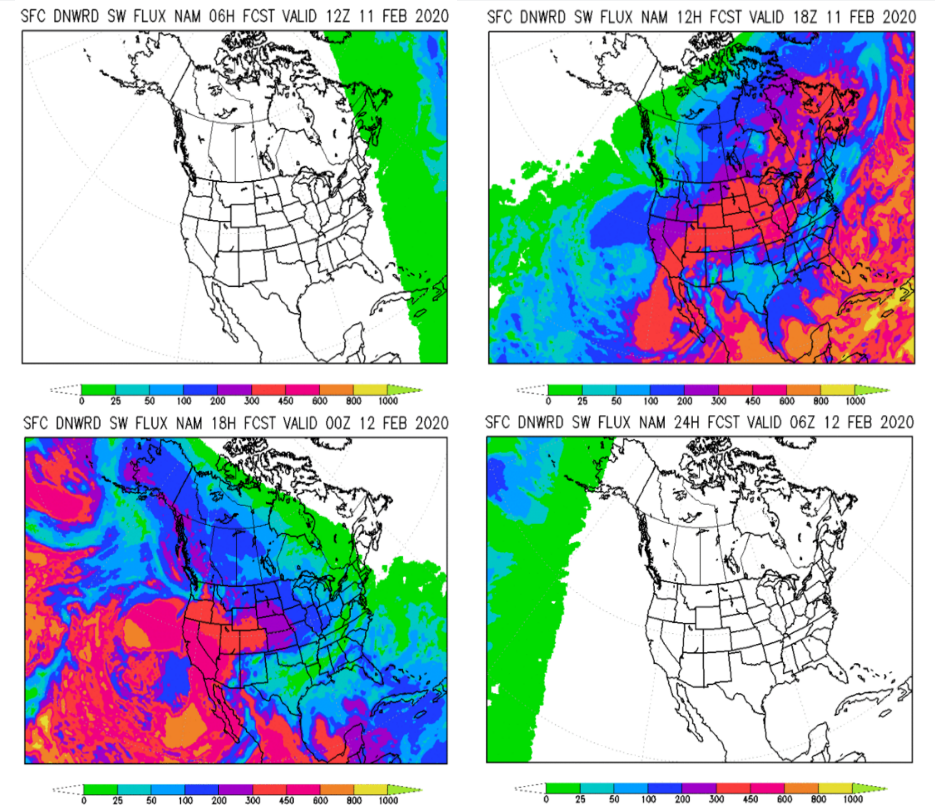
\includegraphics[width=0.85\textwidth]{chapter3/fig_nam_dswrf.png}
    	\caption[Downward shortwave radiation flux parameter for 06h, 12h, 18h, 24h UTC forecasts in a day for NAM model data]{Downward Shortwave Radiation Flux parameter from NAM data over North America domain for 06h forecast (top-left), 12h forecast (top-right), 18h forecast (bottom-left) and 24h forecast (bottom-right) UTC for 11th February, 2020.}
    	\label{fig:fig_nam_dswrf}
    \end{center}
\end{figure}

\par The NAM Forecast System is based on the Weather Research and Forecasting (WRF) model infrastructure, following non-hydrostatic dynamics and thus enabling vertical momentum estimations. It provides high resolution forecasts over North America for a forecast horizon of 84 hours, the first 36 of which are at a one hour temporal resolution, and the remaining thereafter, at a 3 hour temporal resolution. The forecasts are published for a grid spanning approximately $12km$ x $12 km$ across the continental United States, which are released four times daily at 00h, 06h, 12h and 18h UTC.

\par Following the update in 2017, the current version of the NAM model follows Janjic-modified Betts-Miller convection \cite{multimodel_janjic} for parameterization of physical processes, RTM-based longwave and shortwave prediction scheme, and an updated Ferrier-Aligo predictive cloud scheme \cite{multimodel_cloud}. The NWP models cannot resolve weather features and physical processes that occur within a single grid box. Vertical redistribution of heat and moisture can easily occur between mesoscale grids resulting in sub grid-scale variations in convection. The Janjic-modified Betts-Miller convection scheme nudges the temperature and moisture profiles in a grid towards a specific reference profile through repeated observations, thus improving the convection parameterizations in the NAM model by decreasing the convective instability.

\par For convective time scales of the order of 30 minutes to 1 hour, radiative heating rates are negligible. However, for the NAM data which has a forecast length of 84 hours, radiative transfer processes in the clouds need to be taken into consideration as well. In a cloud-free atmosphere, the primary absorbers of shortwave radiation are ozone and water vapour. However, in a cloudy atmosphere, shortwave radiation is more complicated, and a spectrum of radiative frequencies on cloud absorption, reflection and transmission need to be considered \cite{multimodel_rtm}. The NAM models implement the columnar RTM models in this effect, which for each vertical level parameterize the cloud radiative properties.

\par Dozens of parameters are available in a NAM model data grid pertaining to environmental components such as altitude, atmospheric pressure, atmospheric radiation, air temperature, water vapour, atmospheric winds, precipitation, soil properties and cloud cover. The features are spread across 60 vertical levels in a 0 - 3 km layer, and across 39 pressure levels from 50mb to 1000mb at 25mb intervals. From among these parameters, in Fig.~\ref{fig:fig_nam_dswrf}\footnote{NAM forecast snapshots retrieved from: \url{https://www.emc.ncep.noaa.gov/mmb/mmbpll/etapll}}, the averaged downwelling short-wave radiation flux over North America for the four forecasts on 11th February, 2020 is reported.

\subsubchapter{PVLIB Forecast Modeling}
Holmgrem et al \cite{pvlib_Holmgren2018} contributed to building \textit{pvlib-python}\footnote{\url{https://github.com/pvlib/pvlib-python}} an open source, python-based tool, ported from the PVLIB MATLAB toolbox developed at Sandia National Laboratories. This software provides a set of utilities for simulating the performance of the photovoltaic energy systems, with implementations of algorithms related to solar energy. Specifically, it contains components to obtain weather forecast data from NOAA/NCEP/NWS models including the GFS, NAM, RAP, HRRR, and the NDFD, retrieved from the UNIDATA THREDDS servers; and components to convert this weather forecast data into a PV power forecast. 

\par For our experiments, we created a NAM weather forecast dataset for the years of 2017 and 2018, retrieved from the NCEP servers. Meanwhile, \textit{pvlib-python} retrieves NAM CONUS 12km resolution forecasts from the THREDDS servers. The key difference between each of these NAM products is that the former is a full complement of both the pressure level fields and surface-based fields, while the latter is a full complement of just the surface-based fields. The NAM data retrieved and processed by \textit{pvlib-python} consists of the following parameters: air temperature, wind speed, total clouds, low clouds, mid clouds and high clouds. In order to be able to use the \textit{pvlib-python} functionalities on the weather forecast dataset collected by us, equivalent surface-level fields were identified in our weather forecast dataset. Thus, compatibility between the NAM data obtained from both the sources was established, enabling the use of \textit{pvlib-python} functionalities on this engineered dataset.

\par \textit{pvlib-python} software contains components, which are implementations of several theoretical formulations to compute irradiance metrics such as diffuse horizontal irradiance (DHI), direct normal irradiance (DNI) and global horizontal irradiance (GHI) from the weather forecast data. DHI is the amount of solar radiation received by a horizontal surface, which has been scattered by the molecules and particles in the atmosphere. It is the part of the solar radiation which does not belong to the $5^{\circ}$ field of view concentric around the sun, and is typically measured with a pyranometer. DNI is the direct radiation received on a plane normal to the sun over the total solar spectrum. It is an essential component of global irradiance, especially in cloudless conditions, and can be measured with the help of a pyrheliometer. While the solar radiation incident on the earth's atmosphere is relatively constant, various factors such as atmospheric conditions, latitude of the location, season of the year, etc. affect the amount of solar radiation incident on the earth's surface. GHI is the total amount of such terrestrial irradiance which is received by a surface horizontal to the surface of the earth. It can measured with the help of pyranometers, and in general, can be computed from DHI and DNI using the following equation, where $\theta_z$ is the \textit{zenith angle} (the angle between sun and the vertical):
\begin{equation}\label{eq:ghi}
    GHI = DHI + DNI . cos(\theta_z)
\end{equation}

\par Each of these irradiance metrics were computed from the \textit{pvlib-python} compatible dataset using two empirical techniques implemented in the software: Clearsky Scaling, Liu Jordan.


\subsubsection*{Clear-sky Scaling}
\par Global horizontal irradiance can be measured with the help of a pyranometer on a horizontal surface, and thus, is typically the most common type of irradiance measurement. Knowledge of the clear sky conditions (absence of visible clouds), is a key requirement for forecasting all three irradiance metrics. Clear-sky models estimate the terrestrial solar radiation under a cloudless sky from various atmospheric conditions. Such models can be generally validated by comparing the measured irradiance in the clear-sky conditions. 

\par Several parametric models have been proposed in literature to compute these irradiance metrics from environmental conditions such as atmospheric turbidity, fractional sunshine, perceptible water vapor, etc. Ineichen et al \cite{pvlib_ineichen} formulated a model to compute Linke turbidity independent of the airmass, and clear-sky GHI from this metric. Going by Larson et al's \cite{pvlib_larson} work, \textit{pvlib-python} scales global horizontal irradiance on the basis of the total cloud cover and clear-sky GHI according to the following equation, where $GHI_{CS}$ is the clear-sky GHI and TCC is the total cloud cover:
\begin{equation}\label{eq:ghi_cs}
    GHI = GHI_{CS} . [0.35 + 0.65(1 - TCC)]
\end{equation}

\par Maxwell et al \cite{pvlib_disc} introduced the popular \textit{Direct Insolation Simulation Code} (DISC) model to compute cloudy-sky DNI from GHI (in this case, computed with Eq. \ref{eq:ghi_cs}) and other environmental factors. Clearness index is the fraction of the solar radiation transmitted through the atmosphere to strike the earth's surface. DISC model uses empirical relationships between the direct and global components of this measure to estimate the direct beam component. Additionally, the clear-sky DHI component can be evaluated from these irradiance metrics and the solar zenith angle using the equation described in Eq. \ref{eq:ghi}.


\subsubsection*{Liu-Jordan Method}
Decomposition models typically utilize only data pertaining to global radiation to estimate diffuse radiation from global solar irradiation data, as can be seen in the previous subsection. They are based on the atmospheric effects in an isolated place, varying according to time of the year, season and climatic conditions \cite{pvlib_liujordan}. Liu et al proposed one of the earliest and simplest models of radiation, the Liu-Jordan model \cite{pvlib_liujordan2}, which presumes that diffuse radiation intensity is distributed uniformly over the whole sky, and helps estimate diffuse radiation on inclined surfaces. In this model, the diffuse irradiance on a surface tilted towards the equator at an angle $\theta$, where $I_D$ is the diffuse radiation on a horizontal surface is given by the following empirical equation:
\begin{equation}\label{eq:lj_dhi}
    I_{Dt} = I_D . (\frac{1 + cos\theta}{2})
\end{equation}

Liu-Jordan model, though simple, is one of the more accurate among isotropic models for estimating diffuse radiation on inclined surfaces \cite{pvlib_liujordan3}. This model helps determine direct normal irradiance, global horizontal irradiance from properties such as extraterrestrial flux, transmittance, and optical air mass number. It has been observed that the Liu-Jordan model provides a good fit to empirical data under overcast skies, but underestimates the solar radiation on tilted surfaces when used for partially-clear and clear-sky days \cite{pvlib_liujordan4}.

\subchapter{Data Collection and Pre-processing}
\subsubsection*{Weather Forecasts}
\begin{table}[h]
\begin{center}
    \caption{NWP-NAM variables retrieved for solar forecasting}
    \label{Tab:table_nam_variables}
    \begin{tabular}{ c c c}
    	\toprule
    	\textbf{Label} & \textbf{Description} & \textbf{Unit} \\
    	\midrule
    	PRES\_SFC & Air Pressure & $Pa$\\
    	HGT\_SFC & Geopotential Height & $gpm$ \\
    	HGT\_TOA & Height at Planetary Boundary Layer & $gpm$ \\
    	TMP\_SFC & Air Temperature & $K$\\
    	VIS\_SFC & Visibility & $m$\\
    	UGRD\_TOA & U-Component of Wind Speed & $m/s$\\
    	VGRD\_TOA & V-Component of Wind Speed & $m/s$\\
    	DSWRF\_SFC & Downward Short-Wave Radiation Flux & $W/m^2$\\
    	DLWRF\_SFC & Downward Long-Wave Radiation Flux & $W/m^2$\\
    	TCC\_EATM & Total Cloud Cover & $\%$ \\
    	\bottomrule
    \end{tabular}
\end{center}
\end{table}

\par As mentioned in 3.1.1, North America Mesoscale (NAM) model data was collected from the years 2017 and 2018 for experiments. From this data, surface-level parameters as described in Table \ref{Tab:table_nam_variables} were retrieved and analyzed. NAM model projects different weather parameters 84 hours into the future, the first 36 hours of the forecast horizon at a 1-hour temporal resolution, and subsequent 48 hours of the forecast horizon at a 3-hour temporal resolution. In this work, we consider the first 24 hour projections of each of the weather parameters along with their corresponding target pyranometer readings.

\subsubsection*{Temporal Features}
\par In \cite{thesis_zach}, Jones et al. extracted temporal features by parameterizing the \textit{time of day} and \textit{time of year} of the forecasts. These measures were computed by scaling the epoch representing the reference time (in nanoseconds) with the inverse of $8.64e+13$ (number of nanoseconds in a day) and $3.1536e+16$ (number of nanoseconds in a year) respectively. The sine and cosine values of these measures were included, resulting in four temporal features, two each representing the \textit{time of day} and \textit{time of year}. However, this approach fails to capture the cyclicity of the reference time in a particular day, or that of a day in a particular month, in a year. In this work, these parameterizations  were modified to represent the hour in a day and the day in a month respectively. The \textit{time of day} was computed by scaling the number of seconds in the reference time with the inverse of $8.64e+4$ (number of seconds in a day); and the \textit{time of year} was computed by scaling the day of the year with the inverse of $365$ or $366$, depending on whether it is a leap year or not. The sine and cosine values of these measures were added as the temporal features. Additionally, such temporal features of the reference time representing the corresponding target hours were also included in their respective predictors.

\subsubsection*{Irradiance Observations}
\par Georgia Power, in collaboration with the University of Georgia set up a 1MW solar facility in Athens, Georgia. The irradiance observations are obtained from three solar arrays in the solar farm, namely array A, array B and array E, representing a dual-axis tracking array, fixed axis array with 200$^{\circ}$(SW) azimuth, and a single-axis tracking array respectively. Each of the solar arrays are installed with thermopile pyranometers from different manufacturers such as Kipp \& Zonen\footnote{\url{https://www.kippzonen.com/}}, and LICOR\footnote{\url{https://www.licor.com/}}. The thermopile pyranometers have a black absorptive surface which uniformly absorbs the solar radiation across the short-wave solar spectrum, i.e, between 0.2 $\mu m$ and 3 $\mu m$. 

\begin{figure}[ht]
    \begin{center}
    	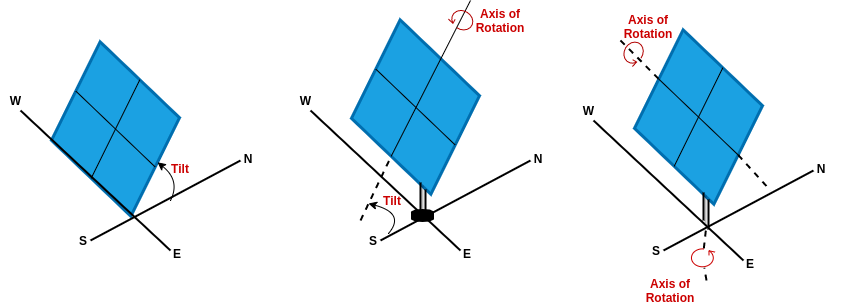
\includegraphics[width=0.85\textwidth]{chapter3/fig_pyranometers.png}
    	\caption[Fixed axis, Single-axis tracking, Dual-axis tracking Solar Arrays]{Fixed axis (left), Single-axis tracking (center), Dual-axis tracking (right) Solar Arrays.}
    	\label{fig:fig_pyranometers}
    \end{center}
\end{figure}

The fixed axis solar array, i.e, array B has limited exposure to the sun, owing to the change in position of the sun during the day from morning to night. Thus, the solar radiation captured by array B is reduced. Though this limitation is negated by installing the fixed solar array at an optimized tilt angle, the solar radiation captured by solar tracking arrays is still considerably higher. In order to maximize the overall solar energy captured, it is necessary to ensure that the angle of incidence of the sunlight on the solar array is constantly perpendicular. This is achieved with the help of single-axis trackers (horizontal and vertical), which have one degree of freedom acting as an axis of rotation; and dual-axis trackers which have two degrees of freedom acting as axes of rotation normal to one another \cite{irradiance_solartracker}. This ability to move along the axes enhances the morning and afternoon performance of the solar tracking systems.

\begin{figure}[ht]
    \begin{center}
    	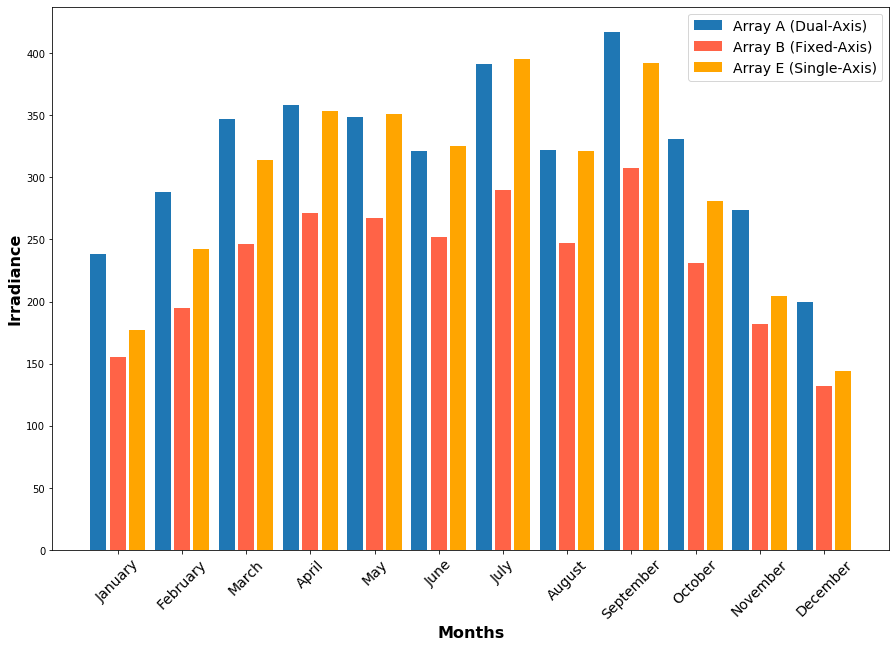
\includegraphics[width=0.85\textwidth]{chapter3/fig_average_irradiance.png}
    	\caption[Average monthly solar radiation captured by arrays A, B and E through 2017.]{Average monthly solar radiation captured by dual-axis (array A), fixed-axis (array B) and single-axis (array E) through 2017.}
    	\label{fig:fig_average_irradiance}
    \end{center}
\end{figure}

While the irradiance observations from the solar arrays are received every five seconds, the NWP NAM model data is available only for four reference times in a day, i.e 00h, 06h, 12h, 18h UTC through 2017 and 2018. Thus, for the target hours in the forecast horizon of all the reference times in 2017 and 2018, for which the NWP NAM model data was collected, the irradiance observations were sampled. In Fig.~\ref{fig:fig_average_irradiance}, the average monthly solar radiation captured by arrays A, B and E through 2017 is shown. It can be observed that the solar radiation captured by the tracking arrays, i.e, array A and array E is consistently higher than that captured by the fixed axis array, i.e array B.

\subsubsection*{Evaluating Impact of Weather Parameters on Irradiance Observations}
\par Mutual information is the measure between two possibly multi-dimensional variables, which quantifies the amount of information obtained from one variable about the other. The relationship detected between the variables can involve either mean, variance or even the higher moments \cite{feature_selection_mi}. The most straightforward and widespread approach towards estimating mutual information follows partitioning the supports of $X$ and $Y$ into bins of finite size, and approximating the sum in the following way:
\begin{equation}\label{eq:eq_mi}
I(X, Y) \approx I_{binned}(X, Y) \equiv \sum_{ij} p(i, j) . log(\frac{p(i, j)}{p_x(i).p_y(j)})
\end{equation}

In this work, the mutual information measure was estimated using the \textit{scikit-learn}\footnote{\url{https://scikit-learn.org/stable/}} machine learning software, which makes use of a non-parametric method based on entropy estimation from the k-nearest neighbors as described in \cite{feature_selection_mi} and \cite{feature_selection_mi2}. Mutual information measure was calculated for the different weather parameters from the NAM data and the irradiance observations from the solar arrays as described in the previous subsections. In Fig. \ref{fig:fig_mi_forecast_target_hr1}, mutual information between different NAM feature projections for the first forecast hour in the forecast horizon, and corresponding irradiance observations from array B is indicated, and their corresponding plots are shown. It can be observed that downward shortwave radiation flux (DSWRF\_SFC), air temperature (TMP\_SFC), height at planetary boundary layer (HGT\_TOA) and total cloud cover (TCC\_EATM) have a mutual information score greater than 0.1, indicating a higher dependency on the irradiance observations. 

\begin{figure}[htbp]
    \begin{center}
    	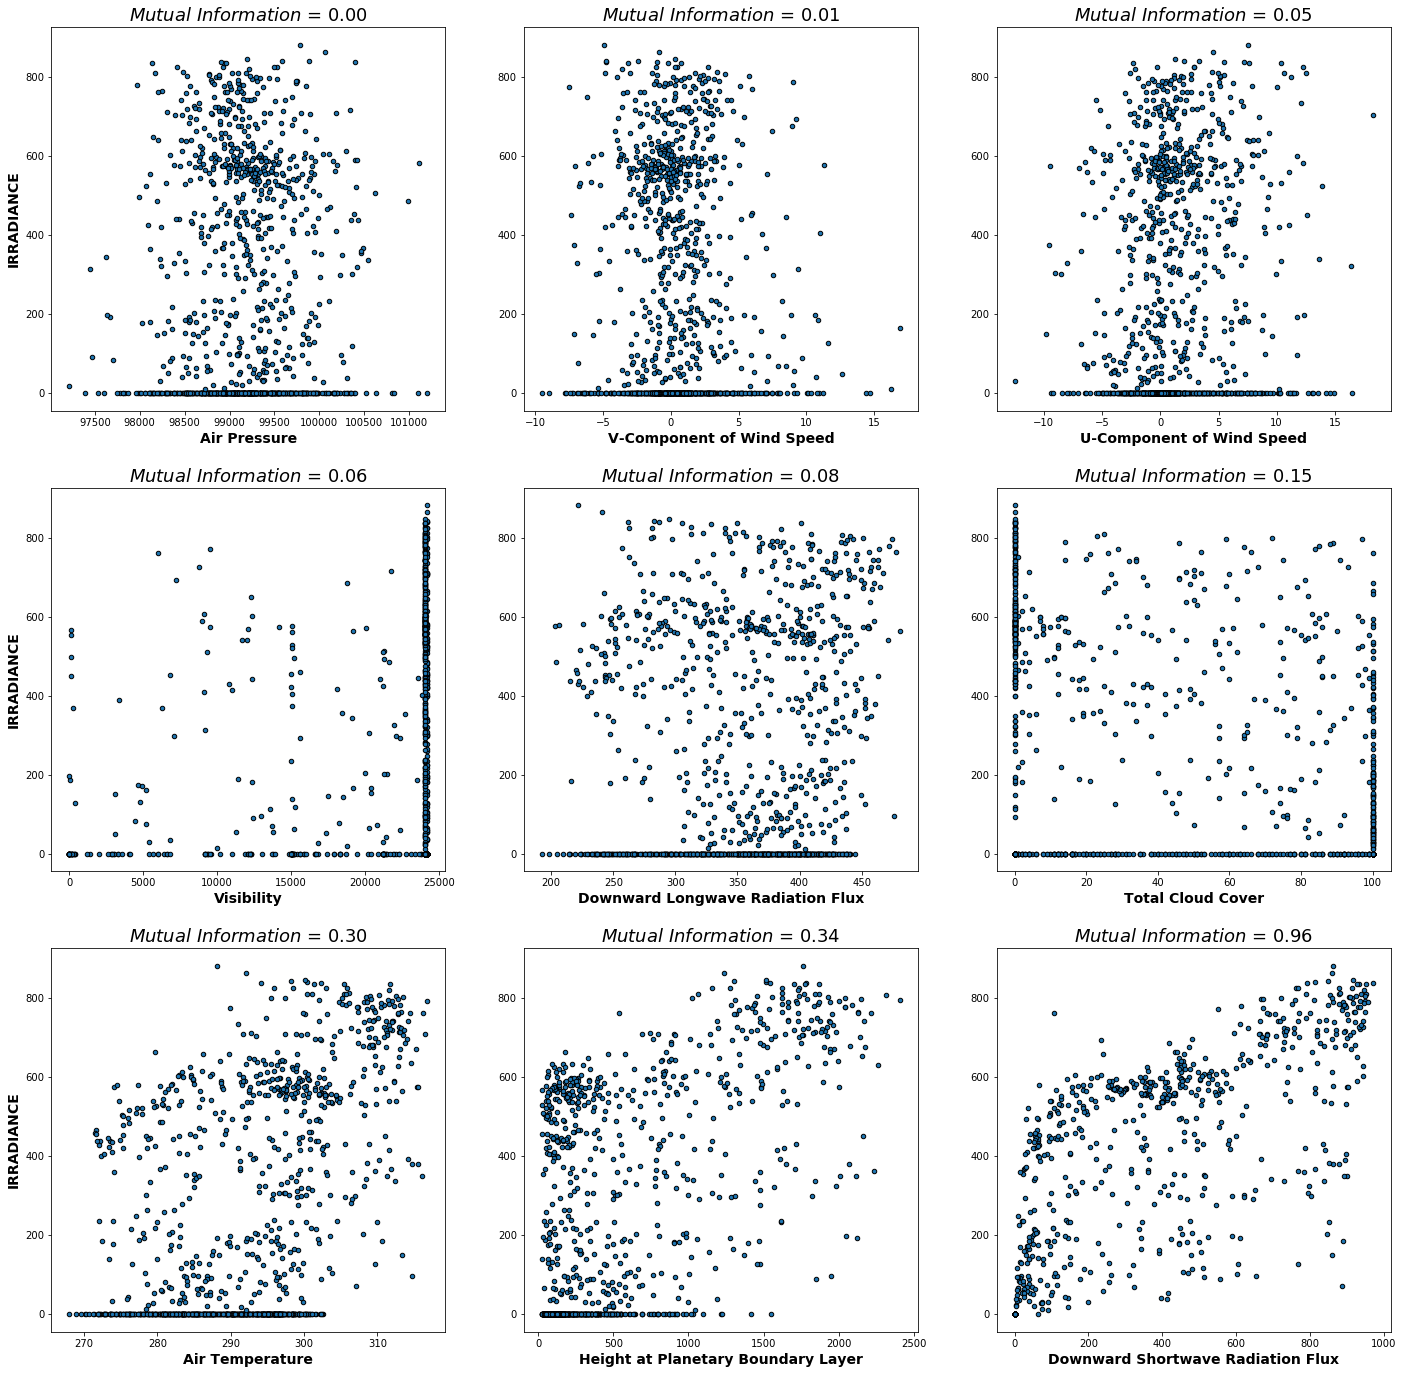
\includegraphics[width=\textwidth]{chapter3/fig_mi_ugabpoa1irr.png}
    	\caption[Mutual information between different NAM weather parameter projections and corresponding solar array B irradiance observations.]{Mutual information between feature projections of different weather parameters in NAM Forecast Model, and the corresponding solar array B irradiance observations.}
    	\label{fig:fig_mi_forecast_target_hr1}
    \end{center}
\end{figure}

\par Downward shortwave radiation flux is the total amount of shortwave radiation that reaches the earth's surface, and is a major component of the total solar radiation on the surface of the earth. Thus, it is the most direct parameter in the estimation solar irradiance, and the high mutual importance score between this weather parameter and the irradiance observations from the solar farm can be justified. By absorbing the incoming solar radiation, the Earth warms up, and its temperature rises. As long as the amount of incoming radiative flux is greater than the outgoing radiative flux, the Earth will continue to warm. Thus, the air temperature at the surface is essential in estimating the amount of heat absorbed at that particular location, which in turn reveals information about the amount of solar radiation absorbed by the thermopiles in the pyranometers. 

\par The influence of clouds on solar irradiance is significant. In the absence of visible clouds, aerosols, precipitable water and other atmospheric conditions affect the transmission of solar radiation through atmosphere. In cloudy conditions though, the clouds absorb a significant amount of the shortwave radiation, making parameters like total cloud cover, which is the fraction of the sky covered by visible clouds essential. The planetary boundary layer (PBL) is the lowest part of the atmosphere which is directly influenced by its contact with the planetary surface. The structure of turbulence within this layer is mainly governed by the PBL height, which is higher during the day, and lower and more stable during nighttime \cite{feature_selection_pbl1}. PBL height characterizes the planetary boundary layer in a fairly integrated manner and affects the weather parameters such as cloud cover and heat flux \cite{feature_selection_pbl2}. This makes PBL height an important parameter in predicting solar irradiance.

\par For the machine learning models to be able to capture and reconstruct the underlying relationship between input-output data pairs effectively, input selection is essential. By removing the redundant and misleading data, input selection often helps in reducing the computational costs and improves the accuracy. Several approaches have been defined in literature for the purpose of input selection, but the most popular technique used for this purpose includes using machine learning models such as the random forests which provide in-built feature selection.

\par Random forests perform a built-in feature selection, because the tree-based strategies used by them naturally rank inputs based on how well they improve the purity of the node. They are an ensemble learning technique constructed over a variety of randomized decision trees, each of which is built over a random extraction of features and data observations. The training of these randomized decision trees is done so that the Gini Impurity is decreased, and those features are selected which help decrease this measure \cite{feature_selection_rf}. Thus, random forests help determine the importance of the features in this manner. It was observed that the weather parameters with higher mutual information scores also received high feature importance scores through this technique, thus validating the dependence of the target irradiance observations on this set of parameters.

\par From among the weather parameters, downward shortwave radiation flux (DSWRF\_SFC), synonymous with global horizontal irradiance (GHI) has the maximum dependency on the target irradiance observations from all the three arrays. In \cite{thesis_zach}, Jones et al. used all 36 feature projections at one-hour temporal resolution for each of the environmental attributes, as the predictor variables for machine learning models. In this work, a forecast horizon of 24 hours was selected, and the relationship between the feature projections in this forecast horizon and the irradiance observations corresponding to the target hours in this forecast horizon was studied. 

\begin{figure}[htb]
    \begin{center}
    	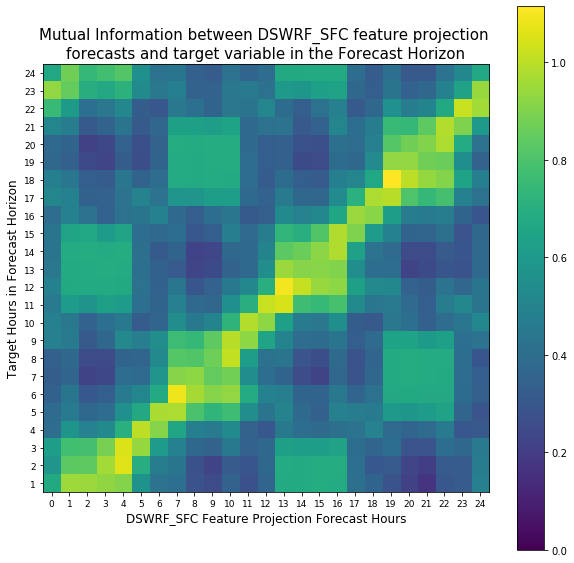
\includegraphics[width=0.65\textwidth]{chapter3/fig_mi_forecast_target.png}
    	\caption[Mutual information between Downward Shortwave Radiation Flux feature projection forecasts and irradiance observations for target hours in the forecast horizon from Solar Array B]{Mutual information between feature projection forecasts of Downward Shortwave Radiation Flux (DSWRF\_SFC) and irradiance observations for target hours in the forecast horizon on Solar Array B.}
    	\label{fig:fig_mi_forecast_target}
    \end{center}
\end{figure}

\par As shown in Fig.~\ref{fig:fig_mi_forecast_target}, it can be observed that the irradiance observations from solar array B for a particular target hour are dependent on only a certain number of feature projections in the forecast horizon. Thus, for each target hour, feature projections from 6 hours ahead, and 6 hours prior were used as predictors. For the first six target hours in the forecast horizon which do not necessarily have six prior feature projections, desired number of feature projections were selected from the end. Similarly, for the last six target hours in the forecast horizon which do not necessarily have six subsequent feature projections, desired number of feature projections were selected from the beginning of the forecast horizon. Such a feature projection selection is justified because it is more likely for the same reference time in two consecutive days to have similar weather conditions. Thus, following this input selections scheme, the NAM model data contributes 13 feature projections for each of the four environmental attributes described earlier, eight temporal features (four for the reference time of the observation, four for the target hour offset from the reference time) towards the post-processing of solar irradiance from each of the solar arrays A, B and E using machine learning models.

\subchapter{Experiment Setup}
\par In this chapter, three series of experiments are performed towards predicting solar irradiance on each of the solar arrays A, B and E. Firstly, solar irradiance forecasting using Numerical Weather Prediction (NWP) models such as North America Mesoscale (NAM) Forecast Model is investigated, replicating the modeling methodology employed in \cite{thesis_zach}. This is compared with the processed NAM dataset obtained, by incorporating the input selection technique described in 3.2. Secondly, a multi-model blending approach is explored, combining the irradiance metrics from NAM Forecast Model and formulations such as Clear-Sky Scaling and Liu-Jordan model in PVLIB. Thirdly, the effect of the spatial expansion of forecast coverage is investigated, by including the weather parameters from a grid of cells around the grid representing Athens. Each of these methodologies are explained in finer detail.

\subsubchapter{Irradiance Forecasting with NAM Weather Forecast Model}
\par In \cite{thesis_zach}, Jones et al. used a variety of machine learning techniques to determine their usefulness in predicting solar irradiance. In the manner described in Section 3.2, North America Mesoscale (NAM) weather forecast data and solar irradiance data from the solar farm at the University of Georgia were collected for the years 2017 and 2018. Planar surface features from the North America Mesoscale (NAM) weather forecast model such as air pressure, geopotential height, height at planetary boundary layer, air temperature, u-component of wind speed, v-component of wind speed, downward shortwave radiation flux and downward longwave radiation flux were used for the purpose of forecasting solar irradiance, 24 hours into the future. The first 36 feature projections of the weather parameters which are at a one-hour temporal resolution were included as the predictor variables for the machine learning models. Additionally, temporal features were considered as well. Models were trained on the data collected during 2017 and evaluated against data collected during 2018.

\par For all machine learning models, finding the ideal set of parameters which define the model architecture, referred to as hyperparameters is paramount. Jones et al performed hyperparameter tuning by carrying out a cross-validated grid search over a parameter space defined around the default hyperparameters given in the \textit{scikit-learn} documentation. The results generated by using these hyperparameters were replicated for the grid representing the NAM forecasts. Following the input selection techniques described in Section 3.2, a new series of machine learning models were trained on the processed NAM dataset. Select feature projections for weather parameters from NAM data such as air temperature, total cloud cover, height at planetary boundary layer and downward shortwave radiation flux were used as predictors for the models, depending on the target hour offset in the forecast horizon. A new set of hyperparameters were picked for these models by performing a randomized cross-validated grid search. These models were trained on data collected during 2017 as well, and evaluated against data collected during 2018. The results obtained by both the methodologies, with and without input selection, were compared and analyzed.

\subsubchapter{Multi-Model Blending Approach }
\par Downward shortwave radiation flux (synonymous with global horizontal irradiance, GHI) was identified to be the most important NAM Weather Forecast Model parameter for solar irradiance forecasting. However, the need to correct the bias in the estimation of this parameter was identified. Irradiance metrics such as global horizontal irradiance (GHI), direct normal irradiance (DNI) and diffuse horizontal irradiance (DHI) can be estimated with the help of several formulations defined in literature. Through the PVLib Forecast Modelling techniques such as Clear-Sky Scaling and Liu-Jordan model, these metrics were estimated from the weather parameters in the NAM data.

\begin{figure}[ht]
    \begin{center}
    	\includegraphics[width=\textwidth]{chapter3/fig_ghi_irradiance.png}
    	\caption[Global horizontal irradiance from NAM data, Clear-sky Scaling and Liu-Jordan against irradiance observations from arrays A, B and E through 2017.]{Global horizontal irradiance from NAM data, Clear-sky Scaling and Liu-Jordan Model against irradiance observations from dual-axis array A (left), fixed-axis array B (center) and single-axis array E (right) through 2017.}
    	\label{fig:fig_ghi_irradiance}
    \end{center}
\end{figure}

\par In this section, a multi-model blending approach is explored, where the weather forecast parameters from NAM are integrated with the irradiance metrics retrieved from Clear-Sky Scaling technique and Liu-Jordan model. Primarily, techniques are explored to combine the GHI parameter from each of the models. In Fig. \ref{fig:fig_ghi_irradiance}, the GHI parameter estimations from each of the models are plotted against the solar irradiance observations from solar arrays A, B and E in the solar farm. 

\subsubsection*{NAM Forecast Model and Clear-Sky Scaling Technique}
The clear-sky scaling technique in \textit{pvlib-python} helps estimate the global horizontal irradiance in clear-sky conditions on the basis of the total cloud cover. Metrics such as clear-sky index help in the removal of diurnal and seasonal signals from a given set of radiation data \cite{expt_clearsky_index}. The clear-sky index for a photovoltaic system can be defined as:\\
\begin{center}
    $K\textsubscript{t} = \frac{GHI\textsubscript{MEAS}}{GHI\textsubscript{CS}}$
\end{center}
where $GHI\textsubscript{MEAS}$ refers to the global horizontal irradiance from a system (which in this case would be $GHI\textsubscript{NAM}$, i.e, global horizontal irradiance from NAM model) and $GHI\textsubscript{CS}$ refers to the global horizontal irradiance from a simulated clear-sky model. The clear-sky index was formulated such that the negative and non-finite values are truncated to zero, and the maximum value is 2, allowing the over-irradiance events typically seen in sub-hourly data.

\begin{figure}[htbp]
    \begin{center}
    	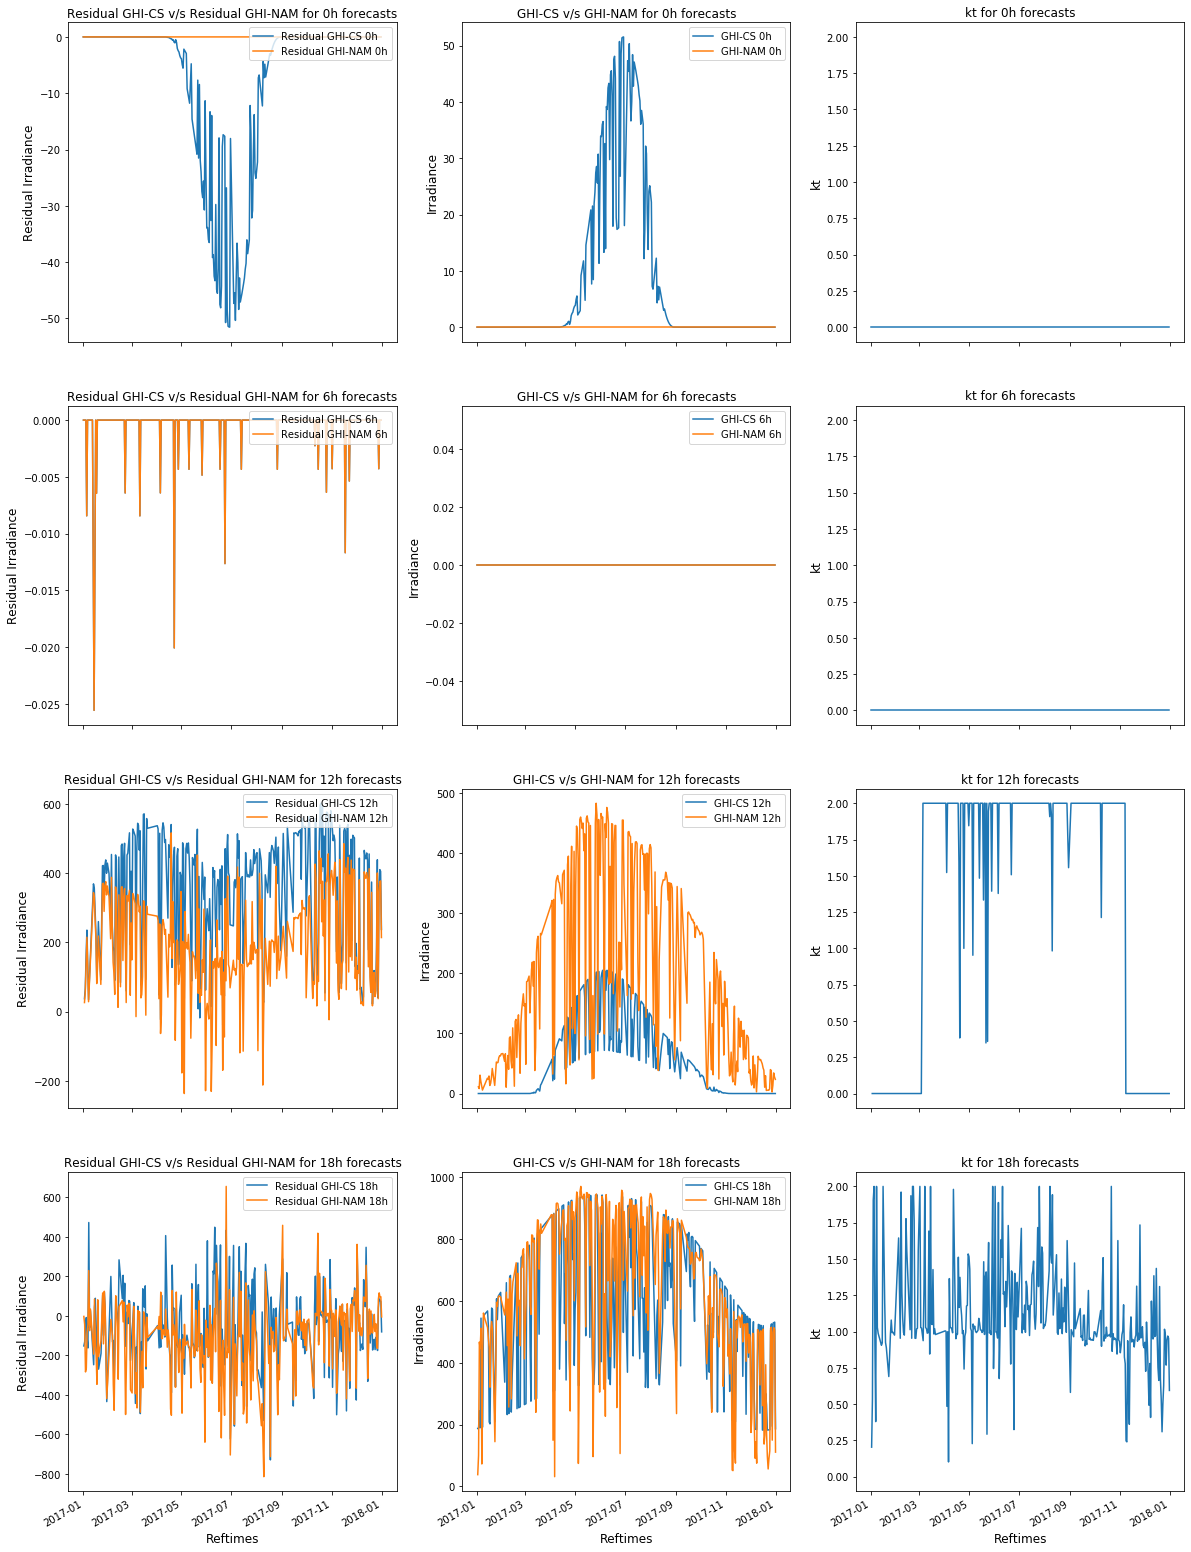
\includegraphics[width=\textwidth]{chapter3/fig_ghi_comparison.png}
    	\caption[Comparing GHI from Clearsky-Scaling ($GHI_{CS}$) and GHI from NAM Forecast Model ($GHI_{NAM}$) for 00h, 06h, 12h, 18h forecasts in 2017]{Comparing GHI from Clearsky-Scaling ($GHI_{CS}$) and GHI from NAM Forecast Model ($GHI_{NAM}$) for 00h, 06h, 12h, 18h forecasts: Residuals of $GHI_{CS}$ and $GHI_{NAM}$ with respect to Array B irradiance observations (left); Clear-sky index ($K_t$) estimations for individual forecasts in 2017 (right).}
    	\label{fig:fig_ghi_comparison}
    \end{center}
\end{figure}

\par In order to assess the $GHI$ values from both NAM model and Clear-Sky Scaling model, residuals between the irradiance observations from solar array B and both $GHI\textsubscript{NAM}$ and $GHI\textsubscript{CS}$ were estimated for the year 2017. Among these, the residuals corresponding to the 00h, 06h, 12h and 18h UTC forecasts were separated, and were plotted in Fig.~\ref{fig:fig_ghi_comparison} (left). The clear-sky index was evaluated for each of the forecasts, and corresponding plots were drawn in Fig.~\ref{fig:fig_ghi_comparison} (right). It was observed that the clear-sky index was constantly zero for the 00h and 06h forecasts throughout the year. This can be attributed to the fact that these forecasts correspond to the time of darkness, resulting in no solar radiation being captured in the solar arrays. Additionally, it can be seen that the residuals for $GHI\textsubscript{NAM}$ are consistently better than the $GHI\textsubscript{CS}$ values for the 12h forecasts, while for the 18h forecasts, they are inconclusive. Thus, the 12h and 18h forecasts were further analyzed with respect to the clear-sky index values.

\begin{table}[h]
\begin{center}
    \caption{MAE of $GHI_{CS}$ and $GHI_{NAM}$ with Array B irradiance for 12h and 18h forecasts.}
    \label{Tab:mean_absolute_residual}
    \begin{tabular}{ c c c c }
    	\toprule
    	\textbf{\parbox{2cm}{\centering Forecast Hour}} & \boldmath\textbf{$K_t$} & \textbf{\parbox{4.5cm}{\centering Mean Absolute Error of \boldmath$GHI_{CS}$}} & \textbf{\parbox{4.5cm}{\centering Mean Absolute Error of \boldmath$GHI_{NAM}$}}\\
    	\midrule
    	\multirow{3}{4em}{$12$} & $< 1.5$ & 271.003 & 219.064 \\ &
    	$> 1.5$ & 383.122 & 204.682 \\
    	\midrule
    	\multirow{3}{4em}{$18$} & $< 1.5$ & 155.63 & 157.38 \\ &
    	$> 1.5$ & 172.869 & 229.998 \\
    	\bottomrule
    \end{tabular}
\end{center}
\end{table}

\par In Table \ref{Tab:mean_absolute_residual}, mean of the absolute values of the residuals (MAE) was computed for the 12h and 18h forecasts, depending on the clear-sky index values estimated for the forecasts. It was observed that for the 12h forecasts, irrespective of $K_t$, $MAD$ corresponding to $GHI_{NAM}$ was lower than that of $GHI_{CS}$, indicating that the GHI predicted by NAM for these forecasts were a better estimation. However, for the 18h forecasts, $MAD$ for forecasts with $K_t < 1.5$ was marginally better for $GHI_{CS}$. Additionally, the $MAD$ for 18h forecasts with $K_t > 1.5$ was significantly better for $GHI_{CS}$, as compared to $GHI_{NAM}$. Thus, it can be concluded that the NAM model tends to overpredict GHI in clear-sky conditions. Thus, in order to correct this bias, for all the 18h forecasts with a $K_t$ value greater than 1.5, $GHI\textsubscript{NAM}$ and $GHI\textsubscript{CS}$ are averaged.

\par From the Clearsky Scaling technique in \textit{pvlib-python}, three irradiance metrics, i.e, GHI, DHI and DNI are retrieved. GHI, which is calculated by scaling total cloud cover, and DNI, which is calculated from the DISC method are highly correlated. Also, DHI, which is empirically calculated from both GHI and DNI, is highly correlated with GHI. Thus, to avoid multicollinearity, the remaining two irradiance metrics, i.e, DHI and DNI are not considered as explanatory variables for the post-processing of irradiance using machine learning models, resulting in the use of only GHI ($GHI_{CS}$) to correct the bias in GHI estimations in NAM model ($GHI_{NAM})$.

\subsubsection*{NAM Forecast Model and Liu-Jordan Model}

The Liu-Jordan Model in \textit{pvlib-python} helps estimate the three irradiance metrics as well. Additionally, this model has been shown to be effective in predicting diffuse irradiance on inclined surfaces. Thus, it was hypothesized that this parameter would help improving irradiance forecasting on solar array A (dual-axis tracking array) and solar array E (single-axis tracking array), which move along their axes based on the position of the sun. In this model, DNI is estimated from transmittance, DHI based on transmittance and solar zenith angle, and GHI is empirically formulated from DHI and DNI. Additionally, it was observed that the GHI observations through this formulation for the year 2017 are highly correlated with DNI. Thus, to avoid multicollinearity amongst the estimators, only GHI and DHI are included along with the estimators from the NAM model for the post-processing of solar irradiance using machine learning models.

\subsubchapter{Geographic Expansion of Forecast Coverage}
Lorenz et al. \cite{expansion_lorenz} found that expanding the forecast region to approximately $100 km$ x $100 km$ and performing a spatial averaging across the region resulted in an improvement in day-ahead solar forecasting. Sanders et. al. \cite{publication_sanders} and Jones et al. \cite{thesis_zach} showed that including the weather forecasts from the grids around the Athens grid resulted in an improved day-ahead solar forecasting as well, though the latter observed that the improvement diminishes as the grid-size grows larger. Additionally, Jones et al also noted that a $3$ x $3$ grid of NAM forecasts centered around Athens, GA, equivalent to a $36km$ x $36km$ area was optimal. A similar geographic expansion of forecast coverage was performed with $3$ x $3$ and $5$ x $5$ grid of NAM forecasts around Athens, GA, resulting in a spatial expansion upto $60km$ x $60km$. The dataset set up using the multi-model blending approach described in 3.3.2, was used to determine the effect of geographic expansion.

\begin{figure}[ht]
    \begin{center}
    	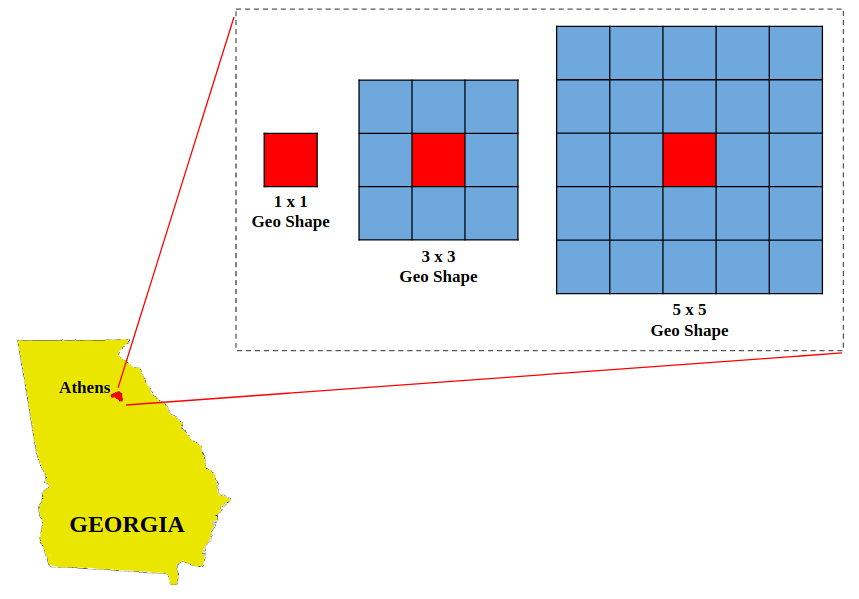
\includegraphics[width=0.65\textwidth]{chapter3/fig_geoshapes.png}
    	\caption[Geographic expansion of forecast coverage around Athens NAM model data grid]{Geographic expansion of forecast coverage with 1 x 1 Geo Shape representing Athens NAM model data grid, 3 x 3 Geo Shape and 5 x 5 Geo Shape representing grid of cells around Athens.}
    	\label{fig:fig_geoshapes}
    \end{center}
\end{figure}

\subchapter{Results and Discussion}
\par In \cite{thesis_zach}, Jones et al used a 24-hour \textit{persistence model} to set a baseline for the more sophisticated machine learning models. In general, persistence models are based on the assumption that conditions remain unchanged between the current time and a future time. The 24-hour persistence models would measure the solar irradiance at a particular time $t$ based on the irradiance value measured at $t-24$. Making use of such a trivial model as a baseline helps in understanding and preparing the data better, by providing a reference for improving the model. Similar 24-hour \textit{persistence models} were used as a baseline in this work as well.

\par Several machine learning algorithms such as least-squares linear regression (LSLR), k-Nearest Neighbors (KNN), Support Vector Regression (SVR), Decision Trees (DT), Random Forests (RF) and Extreme Gradient Boosted Trees (XGBT) were used for the purpose of forecasting. Weather parameter inputs from the NAM data were used as inputs to the machine learning models, and the irradiance observations from the solar arrays A, B and E were used as the target variables. Prediction of target irradiance was done for a forecast horizon of 24 hours, i.e, solar irradiance on each of the arrays was predicted 24 hours into the future, at a one hour temporal resolution. Models were trained on data collected during 2017, and evaluated against data collected during 2018. The performance of the machine learning models were evaluated based on the metrics such as \textit{mean absolute error (MAE)} and $R^2$.  

\par Separate machine learning models were trained for each of the target hour offsets between 1 and 24, and their results were analyzed in two schemes: mean of the evaluations for each forecast hour in the forecast horizon ($Overall$); mean of the evaluations for sets of six forecast hours in the forecast horizon, i.e, $1 - 6$, $7 - 12$, $13 - 18$ and $19 - 24$. Such an analysis helped in realizing the performance of the models specifically for different periods in the day. 

\par In this work, an input selection scheme as described in 3.2 was incorporated towards selecting features for the machine learning models. As a part of this scheme, the key differences between Jones' dataset and the one used in this work, towards training with the machine learning models are as follows: Jones et al hadn't considered the \textit{total cloud cover} parameter in the NAM weather dataset; from among the other surface weather variables used, only air temperature, height at planetary boundary layer and downward shortwave radiation flux were considered; instead of the 36 feature projections for each of the weather variables, select feature projections depending on the target hour offset were chosen; design of the temporal features was different. Based on these differences, the two NAM datasets were used as input to different machine learning models.


\begin{table}[h]
\begin{center}
    \caption{Evaluating performance of machine learning algorithms trained against solar array A using NAM Forecast Model data, with and without input selection.}
    \vspace{0.2cm}
    \label{Tab:fs_array_a}
    \begin{tabular}{@{}p{5.3em}ccccccccc@{}}
    \toprule
    \textbf{Methodology} & \textbf{Metric} & \textbf{Horizon} & \textbf{PER} & \textbf{LSLR} & \textbf{SVR} & \textbf{KNN} & \textbf{DT} & \textbf{RF} & \textbf{XGBT} \\ \cmidrule(l){1-10} 
    \multirow{10}{5em}{Without Input Selection} & \multirow{5}{*}{$MAE$} & $1 - 6$ & \_\_ & \_\_ & \_\_ & \_\_ & \_\_ & \_\_ & \_\_ \\
                                              &                   & $7 - 12$ & \_\_ & \_\_ & \_\_ & \_\_ & \_\_ & \_\_ & \_\_ \\
                                              &                   & $13 - 18$ & \_\_ & \_\_ & \_\_ & \_\_ & \_\_ & \_\_ & \_\_ \\
                                              &                   & $19 - 24$ & \_\_ & \_\_ & \_\_ & \_\_ & \_\_ & \_\_ & \_\_ \\
                                              &                   & $Overall$ & \_\_ & \_\_ & \_\_ & \_\_ & \_\_ & \_\_ & \_\_ \\ \cmidrule(lr){2-10}
                                              & \multirow{5}{*}{$R^2$} & $1 - 6$ & \_\_ & \_\_ & \_\_ & \_\_ & \_\_ & \_\_ & \_\_ \\
                                              &                   & $7 - 12$ & \_\_ & \_\_ & \_\_ & \_\_ & \_\_ & \_\_ & \_\_ \\
                                              &                   & $13 - 18$ & \_\_ & \_\_ & \_\_ & \_\_ & \_\_ & \_\_ & \_\_ \\
                                              &                   & $19 - 24$ & \_\_ & \_\_ & \_\_ & \_\_ & \_\_ & \_\_ & \_\_ \\
                                              &                   & $Overall$ & \_\_ & \_\_ & \_\_ & \_\_ & \_\_ & \_\_ & \_\_ \\ 
    \midrule
    Relative Imp. & $\bigtriangleup MAE$ (\%)  & $Overall$ & $-$ & \_\_ & \_\_ & \_\_ & \_\_ & \_\_ & \_\_ \\ 
    \midrule
    \multirow{10}{5em}{Input Selection}
                                              & \multirow{5}{*}{$MAE$} & $1 - 6$ & \_\_ & \_\_ & \_\_ & \_\_ & \_\_ & \_\_ & \_\_ \\
                                              &                   & $6 - 12$ & \_\_ & \_\_ & \_\_ & \_\_ & \_\_ & \_\_ & \_\_ \\
                                              &                   & $13 - 18$ & \_\_ & \_\_ & \_\_ & \_\_ & \_\_ & \_\_ & \_\_ \\
                                              &                   & $19 - 24$ & \_\_ & \_\_ & \_\_ & \_\_ & \_\_ & \_\_ & \_\_ \\
                                              &                   & $Overall$ & \_\_ & \_\_ & \_\_ & \_\_ & \_\_ & \_\_ & \_\_ \\ \cmidrule(lr){2-10}
                                              & \multirow{5}{*}{$R^2$} & $1 - 6$ & \_\_ & \_\_ & \_\_ & \_\_ & \_\_ & \_\_ & \_\_ \\
                                              &                   & $7 - 12$ & \_\_ & \_\_ & \_\_ & \_\_ & \_\_ & \_\_ & \_\_ \\
                                              &                   & $13 - 18$ & \_\_ & \_\_ & \_\_ & \_\_ & \_\_ & \_\_ & \_\_ \\
                                              &                   & $19 - 24$ & \_\_ & \_\_ & \_\_ & \_\_ & \_\_ & \_\_ & \_\_ \\
                                              &                   & $Overall$ & \_\_ & \_\_ & \_\_ & \_\_ & \_\_ & \_\_ & \_\_ \\ 
    \bottomrule
    \end{tabular}
\end{center}
\end{table}

\begin{table}[h]
\begin{center}
    \caption{Evaluating performance of machine learning algorithms trained against solar array B using NAM Forecast Model data, with and without input selection.}
    \vspace{0.2cm}
    \begin{tabular}{@{}p{5.3em}ccccccccc@{}}
    \toprule
    \textbf{Methodology} & \textbf{Metric} & \textbf{Horizon} & \textbf{PER} & \textbf{LSLR} & \textbf{SVR} & \textbf{KNN} & \textbf{DT} & \textbf{RF} & \textbf{XGBT} \\ \cmidrule(l){1-10} 
    \multirow{10}{5em}{Without Input Selection} & \multirow{5}{*}{$MAE$} & $1 - 6$ & \_\_ & \_\_ & \_\_ & \_\_ & \_\_ & \_\_ & \_\_ \\
                                              &                   & $7 - 12$ & \_\_ & \_\_ & \_\_ & \_\_ & \_\_ & \_\_ & \_\_ \\
                                              &                   & $13 - 18$ & \_\_ & \_\_ & \_\_ & \_\_ & \_\_ & \_\_ & \_\_ \\
                                              &                   & $19 - 24$ & \_\_ & \_\_ & \_\_ & \_\_ & \_\_ & \_\_ & \_\_ \\
                                              &                   & $Overall$ & \_\_ & \_\_ & \_\_ & \_\_ & \_\_ & \_\_ & \_\_ \\ \cmidrule(lr){2-10}
                                              & \multirow{5}{*}{$R^2$} & $1 - 6$ & \_\_ & \_\_ & \_\_ & \_\_ & \_\_ & \_\_ & \_\_ \\
                                              &                   & $7 - 12$ & \_\_ & \_\_ & \_\_ & \_\_ & \_\_ & \_\_ & \_\_ \\
                                              &                   & $13 - 18$ & \_\_ & \_\_ & \_\_ & \_\_ & \_\_ & \_\_ & \_\_ \\
                                              &                   & $19 - 24$ & \_\_ & \_\_ & \_\_ & \_\_ & \_\_ & \_\_ & \_\_ \\
                                              &                   & $Overall$ & \_\_ & \_\_ & \_\_ & \_\_ & \_\_ & \_\_ & \_\_ \\ 
    \midrule
    Relative Imp. & $\bigtriangleup MAE$ (\%)  & $Overall$ & $-$ & \_\_ & \_\_ & \_\_ & \_\_ & \_\_ & \_\_ \\ 
    \midrule
    \multirow{10}{5em}{Input Selection}
                                              & \multirow{5}{*}{$MAE$} & $1 - 6$ & \_\_ & \_\_ & \_\_ & \_\_ & \_\_ & \_\_ & \_\_ \\
                                              &                   & $6 - 12$ & \_\_ & \_\_ & \_\_ & \_\_ & \_\_ & \_\_ & \_\_ \\
                                              &                   & $13 - 18$ & \_\_ & \_\_ & \_\_ & \_\_ & \_\_ & \_\_ & \_\_ \\
                                              &                   & $19 - 24$ & \_\_ & \_\_ & \_\_ & \_\_ & \_\_ & \_\_ & \_\_ \\
                                              &                   & $Overall$ & \_\_ & \_\_ & \_\_ & \_\_ & \_\_ & \_\_ & \_\_ \\ \cmidrule(lr){2-10}
                                              & \multirow{5}{*}{$R^2$} & $1 - 6$ & \_\_ & \_\_ & \_\_ & \_\_ & \_\_ & \_\_ & \_\_ \\
                                              &                   & $7 - 12$ & \_\_ & \_\_ & \_\_ & \_\_ & \_\_ & \_\_ & \_\_ \\
                                              &                   & $13 - 18$ & \_\_ & \_\_ & \_\_ & \_\_ & \_\_ & \_\_ & \_\_ \\
                                              &                   & $19 - 24$ & \_\_ & \_\_ & \_\_ & \_\_ & \_\_ & \_\_ & \_\_ \\
                                              &                   & $Overall$ & \_\_ & \_\_ & \_\_ & \_\_ & \_\_ & \_\_ & \_\_ \\ 
    \bottomrule
    \end{tabular}
\end{center}
\end{table}

\begin{table}[h]
\begin{center}
    \caption{Evaluating performance of machine learning algorithms trained against solar array E using NAM Forecast Model data, with and without input selection.}
    \vspace{0.2cm}
    \begin{tabular}{@{}p{5.3em}ccccccccc@{}}
    \toprule
    \textbf{Methodology} & \textbf{Metric} & \textbf{Horizon} & \textbf{PER} & \textbf{LSLR} & \textbf{SVR} & \textbf{KNN} & \textbf{DT} & \textbf{RF} & \textbf{XGBT} \\ \cmidrule(l){1-10} 
    \multirow{10}{5em}{Without Input Selection} & \multirow{5}{*}{$MAE$} & $1 - 6$ & \_\_ & \_\_ & \_\_ & \_\_ & \_\_ & \_\_ & \_\_ \\
                                              &                   & $7 - 12$ & \_\_ & \_\_ & \_\_ & \_\_ & \_\_ & \_\_ & \_\_ \\
                                              &                   & $13 - 18$ & \_\_ & \_\_ & \_\_ & \_\_ & \_\_ & \_\_ & \_\_ \\
                                              &                   & $19 - 24$ & \_\_ & \_\_ & \_\_ & \_\_ & \_\_ & \_\_ & \_\_ \\
                                              &                   & $Overall$ & \_\_ & \_\_ & \_\_ & \_\_ & \_\_ & \_\_ & \_\_ \\ \cmidrule(lr){2-10}
                                              & \multirow{5}{*}{$R^2$} & $1 - 6$ & \_\_ & \_\_ & \_\_ & \_\_ & \_\_ & \_\_ & \_\_ \\
                                              &                   & $7 - 12$ & \_\_ & \_\_ & \_\_ & \_\_ & \_\_ & \_\_ & \_\_ \\
                                              &                   & $13 - 18$ & \_\_ & \_\_ & \_\_ & \_\_ & \_\_ & \_\_ & \_\_ \\
                                              &                   & $19 - 24$ & \_\_ & \_\_ & \_\_ & \_\_ & \_\_ & \_\_ & \_\_ \\
                                              &                   & $Overall$ & \_\_ & \_\_ & \_\_ & \_\_ & \_\_ & \_\_ & \_\_ \\ 
    \midrule
    Relative Imp. & $\bigtriangleup MAE$ (\%)  & $Overall$ & $-$ & \_\_ & \_\_ & \_\_ & \_\_ & \_\_ & \_\_ \\ 
    \midrule
    \multirow{10}{5em}{Input Selection}
                                              & \multirow{5}{*}{$MAE$} & $1 - 6$ & \_\_ & \_\_ & \_\_ & \_\_ & \_\_ & \_\_ & \_\_ \\
                                              &                   & $6 - 12$ & \_\_ & \_\_ & \_\_ & \_\_ & \_\_ & \_\_ & \_\_ \\
                                              &                   & $13 - 18$ & \_\_ & \_\_ & \_\_ & \_\_ & \_\_ & \_\_ & \_\_ \\
                                              &                   & $19 - 24$ & \_\_ & \_\_ & \_\_ & \_\_ & \_\_ & \_\_ & \_\_ \\
                                              &                   & $Overall$ & \_\_ & \_\_ & \_\_ & \_\_ & \_\_ & \_\_ & \_\_ \\ \cmidrule(lr){2-10}
                                              & \multirow{5}{*}{$R^2$} & $1 - 6$ & \_\_ & \_\_ & \_\_ & \_\_ & \_\_ & \_\_ & \_\_ \\
                                              &                   & $7 - 12$ & \_\_ & \_\_ & \_\_ & \_\_ & \_\_ & \_\_ & \_\_ \\
                                              &                   & $13 - 18$ & \_\_ & \_\_ & \_\_ & \_\_ & \_\_ & \_\_ & \_\_ \\
                                              &                   & $19 - 24$ & \_\_ & \_\_ & \_\_ & \_\_ & \_\_ & \_\_ & \_\_ \\
                                              &                   & $Overall$ & \_\_ & \_\_ & \_\_ & \_\_ & \_\_ & \_\_ & \_\_ \\ 
    \bottomrule
    \end{tabular}
\end{center}
\end{table}


\begin{table}[h]
\begin{center}
    \caption{Sample Table 1}
    \begin{tabular}{ c c c c c c c c c}
    	\toprule
    	\textbf{Metric} & \textbf{Horizon} & \textbf{PER} & \textbf{LSLR} & \textbf{SVR} & \textbf{KNN} & \textbf{DT} & \textbf{RF} & \textbf{XGBT}\\
    	\midrule
    	\multirow{3}{4em}{$MAE$} & $1 - 6$ & \_\_ & \_\_ & \_\_ & \_\_ & \_\_ & \_\_ & \_\_\\ &
    	$7 - 12$ & \_\_ & \_\_ & \_\_ & \_\_ & \_\_ & \_\_ & \_\_\\ &
    	$13 - 18$ & \_\_ & \_\_ & \_\_ & \_\_ & \_\_ & \_\_ & \_\_\\ &
    	$19 - 24$ & \_\_ & \_\_ & \_\_ & \_\_ & \_\_ & \_\_ & \_\_\\ &
    	$Overall$ & \_\_ & \_\_ & \_\_ & \_\_ & \_\_ & \_\_ & \_\_\\
    	\midrule
    	\multirow{3}{4em}{$R^2$} & $1 - 6$ & \_\_ & \_\_ & \_\_ & \_\_ & \_\_ & \_\_ & \_\_ \\ &
    	$7 - 12$ & \_\_ & \_\_ & \_\_ & \_\_ & \_\_ & \_\_ & \_\_\\ &
    	$13 - 18$ & \_\_ & \_\_ & \_\_ & \_\_ & \_\_ & \_\_ & \_\_\\ &
    	$19 - 24$ & \_\_ & \_\_ & \_\_ & \_\_ & \_\_ & \_\_ & \_\_\\ &
    	$Overall$ & \_\_ & \_\_ & \_\_ & \_\_ & \_\_ & \_\_ & \_\_\\
    	\bottomrule
    \end{tabular}
\end{center}
\end{table}

\begin{table}[h]
\begin{center}
    \caption{Sample Table 2}
    \begin{tabular}{l l l l l l l l l l l}
        \toprule
        \multirow{2}{*}{\textbf{Metric}} & \multirow{2}{*}{\textbf{Horizon}} & \multicolumn{3}{c}{\textbf{KNN}} & \multicolumn{3}{c}{\textbf{RF}} & \multicolumn{3}{c}{\textbf{XGBT}}\\
        \cmidrule{3-11}
         &  & 1x1 & 3x3 & 5x5 & 1x1 & 3x3 & 5x5 & 1x1 & 3x3 & 5x5 \\
        \midrule
        \multirow{5}{*}{$MAE$} & $1 - 6$ & \_ & \_ & \_ & \_ & \_ & \_ & \_ & \_ & \_ \\
        & $7 - 12$ & \_ & \_ & \_ & \_ & \_ & \_ & \_ & \_ & \_ \\
        & $13 - 18$ & \_ & \_ & \_ & \_ & \_ & \_ & \_ & \_ & \_ \\
        & $19 - 24$ & \_ & \_ & \_ & \_ & \_ & \_ & \_ & \_ & \_ \\
        & $Overall$ & \_ & \_ & \_ & \_ & \_ & \_ & \_ & \_ & \_ \\
        \midrule
        \multirow{5}{*}{$R^2$} & $1 - 6$ & \_ & \_ & \_ & \_ & \_ & \_ & \_ & \_ & \_ \\
        & $7 - 12$ & \_ & \_ & \_ & \_ & \_ & \_ & \_ & \_ & \_ \\
        & $13 - 18$ & \_ & \_ & \_ & \_ & \_ & \_ & \_ & \_ & \_ \\
        & $19 - 24$ & \_ & \_ & \_ & \_ & \_ & \_ & \_ & \_ & \_ \\
        & $Overall$ & \_ & \_ & \_ & \_ & \_ & \_ & \_ & \_ & \_ \\
        \bottomrule
    \end{tabular}
\end{center}
\end{table}

\newpage
\chapter{}{{Multi-Model Approach to Solar Irradiance Forecasting}}{Multi-Model Blending Approach to Solar Irradiance Forecasting}

\subchapter{Overview}
\par Downward shortwave radiation flux, synonymous with global horizontal irradiance (GHI) is measured by NWP models using columnar radiative transfer models (RTM). The RTMs help in determining cloud optical properties for different wavelength bands with the help of weather variables such as air temperature, gas concentrations and cloud structure. These cloud properties are essential for effective cloud modeling as they determine the absorption, scattering and reflection of global solar radiation. Thus, they contribute to effective shortwave radiation flux computation. However, the direct output from the mesoscale models has shown severe deviations between forecasted and real irradiance \cite{multimodel_ghi}. 

\par While the usage of additional weather variables in machine learning models have shown to improve the post-processing of NWP models by incorporating site-specific information, it has to be taken into consideration that there is a significant variability in the GHI measured by the NWP models with respect to the cloud conditions. Mathiesan et al \cite{multimodel_overpredict} found that the NAM Forecast model tends to overpredict GHI in clear-sky conditions, i.e. conditions in which visible clouds are absent, by up to 40 percent. Thus, effectively identifying the clear-sky conditions becomes essential, following which the bias in GHI measured by the NAM Forecast System in these conditions can be corrected.

\par There are multiple empirical solar radiation formulations which have been extensively discussed in literature \cite{litrev_pvlib10}\cite{litrev_pvlib11}\cite{litrev_pvlib12}\cite{litrev_pvlib13}\cite{litrev_pvlib14}\cite{litrev_pvlib9}, which compute the irradiance metrics from environmental conditions such as cloud cover. These can be broadly classified into decomposition models and parametric models. Using assumptions on solar geometry and transmittance, the former are used to estimate direct beam and diffuse irradiance. The latter are useful for approximating daily solar radiation reaching tilted surfaces. GHI can be empirically estimated from these irradiance metrics. In this \restoregeometry\noindent section, two such empirical solar radiation models, \textit{Clear-Sky Scaling} and \textit{Liu-Jordan Model} are discussed, which help estimate GHI, DHI and DNI. Using measures such as clear-sky index which is useful to separate clear-sky conditions from cloudy conditions; and clearness index, which is the measure of clearness of the atmosphere, GHI measured by NAM Forecast System can be empirically corrected in conditions where visible clouds are absent.

\subchapter{Empirical Solar Radiation Models}
\par Solar researchers have developed various empirical formulations which help in determining the relation between different components of solar radiation and various meteorological parameters. These can be broadly classified into \textit{decomposition} and \textit{parametric} models. The parametric models require information about atmospheric conditions such as turbidity, cloud cover, etc. to be able to formulate the different components of solar irradiance such as diffuse horizontal irradiance (DHI), direct normal irradiance (DNI) and global horizontal irradiance (GHI). Decomposition models formulate equations to estimate the solar irradiance components based on the corerlations between them. Such formulations are relevant, especially in cases where meteorological data is not adequately available.

\par DHI is the amount of solar radiation received by a horizontal surface, which has been scattered by the molecules and particles in the atmosphere. It is the part of the solar radiation which does not belong to the $5^{\circ}$ field of view concentric around the sun, and is typically measured with a pyranometer. DNI is the direct radiation received on a plane normal to the sun over the total solar spectrum. It is an essential component of global irradiance, especially in cloudless conditions, and can be measured with the help of a pyrheliometer. While the solar radiation incident on the earth's atmosphere is relatively constant, various factors such as atmospheric conditions, latitude of the location, season of the year, etc. affect the amount of solar radiation incident on the earth's surface. GHI is the total amount of such terrestrial irradiance which is received by a surface horizontal to the surface of the earth. It can measured with the help of pyranometers, and in general, can be computed from DHI and DNI using the following equation, where $\theta_z$ is the \textit{zenith angle} (the angle between sun and the vertical):
\begin{equation}\label{eq:ghi}
    GHI = DHI + DNI . cos(\theta_z)
\end{equation}

\par Holmgrem et al \cite{pvlib_Holmgren2018} contributed to building \textit{pvlib-python}\footnote{\url{https://github.com/pvlib/pvlib-python}} an open source, python-based tool, ported from the PVLIB MATLAB toolbox developed at Sandia National Laboratories. This software provides a set of utilities for simulating the performance of the photovoltaic energy systems, with implementations of algorithms related to solar energy. Specifically, it contains components to obtain weather forecast data from NOAA/NCEP/NWS models including the GFS, NAM, RAP, HRRR, and the NDFD, retrieved from the UNIDATA THREDDS servers; and components to convert this weather forecast data into a PV power forecast. 

\par For our experiments, we created a NAM weather forecast dataset for the years of 2017 and 2018, retrieved from the NCEP servers. Meanwhile, \textit{pvlib-python} retrieves NAM CONUS 12km resolution forecasts from the THREDDS servers. The key difference between each of these NAM products is that the former is a full complement of both the pressure level fields and surface-based fields, while the latter is a full complement of just the surface-based fields. The NAM data retrieved and processed by \textit{pvlib-python} consists of the following parameters: air temperature, wind speed, total clouds, low clouds, mid clouds and high clouds. In order to be able to use the \textit{pvlib-python} functionalities on the weather forecast dataset collected by us, equivalent surface-level fields were identified in our weather forecast dataset. Thus, compatibility between the NAM data obtained from both the sources was established, enabling the use of \textit{pvlib-python} functionalities on this engineered dataset.

\par \textit{pvlib-python} software contains components, which are implementations of several theoretical formulations to compute irradiance metrics such as DHI, DNI and GHI from the weather forecast data. In this work, each of these irradiance metrics were computed from the \textit{pvlib-python} compatible NAM dataset using two empirical techniques implemented in the software: Clearsky Scaling, Liu-Jordan Model.

\subsubchapter{Clear-sky Scaling}
\par Global horizontal irradiance can be measured with the help of a pyranometer on a horizontal surface, and thus, is typically the most common type of irradiance measurement. Knowledge of the clear sky conditions (absence of visible clouds), is a key requirement for forecasting all three irradiance metrics. Clear-sky models estimate the terrestrial solar radiation under a cloudless sky from various atmospheric conditions. Such models can be generally validated by comparing the measured irradiance in the clear-sky conditions. 

\par Several parametric models have been proposed in literature to compute these irradiance metrics from environmental conditions such as atmospheric turbidity, fractional sunshine, perceptible water vapor, etc. Ineichen et al \cite{pvlib_ineichen} formulated a model to compute Linke turbidity independent of the airmass, and clear-sky GHI from this metric. Going by Larson et al's \cite{pvlib_larson} work, \textit{pvlib-python} scales global horizontal irradiance on the basis of the total cloud cover and clear-sky GHI according to the following equation, where $GHI_{CS}$ is the clear-sky GHI and TCC is the total cloud cover:
\begin{equation}\label{eq:ghi_cs}
    GHI = GHI_{CS} . [0.35 + 0.65(1 - TCC)]
\end{equation}

\par Maxwell et al \cite{pvlib_disc} introduced the popular \textit{Direct Insolation Simulation Code} (DISC) model to compute cloudy-sky DNI from GHI (in this case, computed with Eq. \ref{eq:ghi_cs}) and other environmental factors. Clearness index is the fraction of the solar radiation transmitted through the atmosphere to strike the earth's surface. DISC model uses empirical relationships between the direct and global components of this measure to estimate the direct beam component. Additionally, the clear-sky DHI component can be evaluated from these irradiance metrics and the solar zenith angle using the equation described in Eq. \ref{eq:ghi}.

\subsubchapter{Liu-Jordan Model}
Decomposition models typically utilize only data pertaining to global radiation to estimate diffuse radiation from global solar irradiation data, as can be seen in the previous subsection. They are based on the atmospheric effects in an isolated place, varying according to time of the year, season and climatic conditions \cite{pvlib_liujordan}. Liu et al proposed one of the earliest and simplest models of radiation, the Liu-Jordan model \cite{pvlib_liujordan2}, which presumes that diffuse radiation intensity is distributed uniformly over the whole sky, and helps estimate diffuse radiation on inclined surfaces. In this model, the diffuse irradiance on a surface tilted towards the equator at an angle $\theta$, where $I_D$ is the diffuse radiation on a horizontal surface is given by the following empirical equation:
\begin{equation}\label{eq:lj_dhi}
    I_{Dt} = I_D . (\frac{1 + cos\theta}{2})
\end{equation}

Liu-Jordan model, though simple, is one of the more accurate among isotropic models for estimating diffuse radiation on inclined surfaces \cite{pvlib_liujordan3}. This model helps determine direct normal irradiance, global horizontal irradiance from properties such as extraterrestrial flux, transmittance, and optical air mass number. It has been observed that the Liu-Jordan model provides a good fit to empirical data under overcast skies, but underestimates the solar radiation on tilted surfaces when used for partially-clear and clear-sky days \cite{pvlib_liujordan4}.

\subchapter{Experiment Setup}
\par In this chapter, three series of experiments are performed towards predicting solar irradiance on each of the solar arrays A, B and E. Firstly, solar irradiance forecasting using Numerical Weather Prediction (NWP) models such as North America Mesoscale (NAM) Forecast Model is investigated, replicating the modeling methodology employed in \cite{thesis_zach}. This is compared with the processed NAM dataset obtained, by incorporating the input selection technique described in 3.2. Secondly, a multi-model blending approach is explored, combining the irradiance metrics from NAM Forecast Model and formulations such as Clear-Sky Scaling and Liu-Jordan model in PVLIB. Thirdly, the effect of the spatial expansion of forecast coverage is investigated, by including the weather parameters from a grid of cells around the grid representing Athens. Each of these methodologies are explained in finer detail.

\par Downward shortwave radiation flux (synonymous with global horizontal irradiance, GHI) was identified to be the most important NAM Weather Forecast Model parameter for solar irradiance forecasting. However, a need to correct the bias in the estimation of this parameter was identified. Irradiance metrics such as global horizontal irradiance (GHI), direct normal irradiance (DNI) and diffuse horizontal irradiance (DHI) can be estimated with the help of several formulations defined in literature. With the help of implementations of empirical solar radiation models such as Clear-Sky Scaling and Liu-Jordan model in \textit{pvlib python}, these metrics were estimated from the weather parameters in the NAM data.

\begin{figure}[ht]
    \begin{center}
    	\includegraphics[width=\textwidth]{chapter4/fig_ghi_irradiance.png}
    	\caption[Global horizontal irradiance from NAM data, Clear-sky Scaling and Liu-Jordan against irradiance observations from arrays A, B and E through 2017.]{Global horizontal irradiance from NAM data, Clear-sky Scaling and Liu-Jordan Model against irradiance observations from dual-axis array A (left), fixed-axis array B (center) and single-axis array E (right) through 2017.}
    	\label{fig:fig_ghi_irradiance}
    \end{center}
\end{figure}

\par In this section, a multi-model blending approach is explored, where the weather forecast parameters from NAM are integrated with the irradiance metrics retrieved from Clear-Sky Scaling technique and Liu-Jordan model. Primarily, techniques are explored to combine the GHI parameter from each of the models based on measures such as \textit{clear-sky index} and \textit{clearness index} which are described in greater detail in the following sections. In Fig. \ref{fig:fig_ghi_irradiance}, the GHI parameter estimations from each of the models are plotted against the solar irradiance observations from the dual-axis tracking solar array (array A), fixed-axis solar array (array B) and single-axis solar array (array E) in the solar farm. 

\subsubchapter{Blending NAM Forecast Model and Clear-Sky Scaling Technique}
The clear-sky scaling technique in \textit{pvlib-python} helps estimate the global horizontal irradiance in clear-sky conditions on the basis of the total cloud cover. Metrics such as clear-sky index help in the removal of diurnal and seasonal signals from a given set of radiation data \cite{expt_clearsky_index}. The clear-sky index for a photovoltaic system can be defined as:\\
\begin{center}
    $K\textsubscript{c} = \frac{GHI\textsubscript{MEAS}}{GHI\textsubscript{CS}}$
\end{center}
where $GHI\textsubscript{MEAS}$ refers to the global horizontal irradiance from a system (which in this case would be $GHI\textsubscript{NAM}$, i.e, global horizontal irradiance from NAM model) and $GHI\textsubscript{CS}$ refers to the global horizontal irradiance from a simulated clear-sky model. The clear-sky index was formulated such that the negative and non-finite values are truncated to zero, and the maximum value is 2, allowing the over-irradiance events typically seen in sub-hourly data.

\begin{figure}[htbp]
    \begin{center}
    	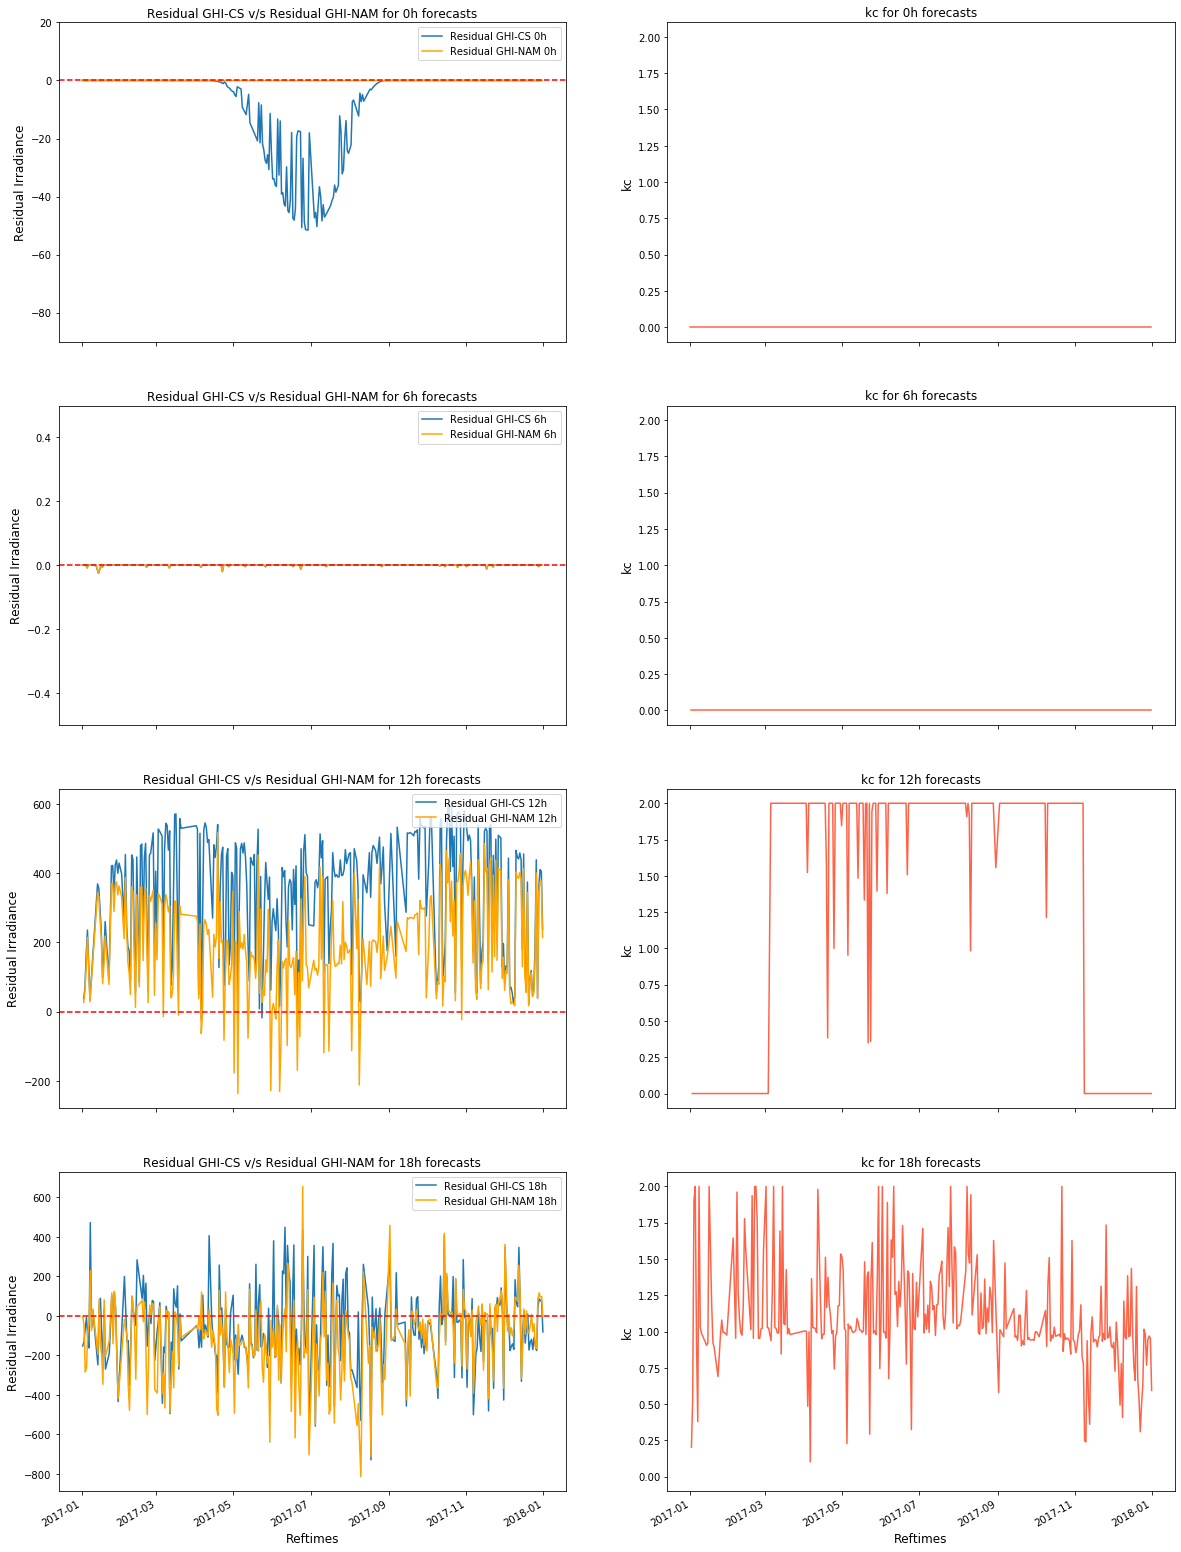
\includegraphics[width=\textwidth]{chapter4/fig_ghi_comparison_cs.png}
    	\caption[Comparing GHI from Clearsky-Scaling ($GHI_{CS}$) and GHI from NAM Forecast Model ($GHI_{NAM}$) for 00h, 06h, 12h, 18h forecasts in 2017]{Comparing GHI from Clearsky-Scaling ($GHI_{CS}$) and GHI from NAM Forecast Model ($GHI_{NAM}$) for 00h, 06h, 12h, 18h forecasts: Residuals of $GHI_{CS}$ and $GHI_{NAM}$ with respect to Array B irradiance observations (left); Clear-sky index ($K_c$) estimations for individual forecasts in 2017 (right).}
    	\label{fig:fig_ghi_comparison_cs}
    \end{center}
\end{figure}

\par In order to assess the $GHI$ values from both NAM model and Clear-Sky Scaling model, residuals between the irradiance observations from solar array B and both $GHI\textsubscript{NAM}$ and $GHI\textsubscript{CS}$ were estimated for the year 2017. Among these, the residuals corresponding to the 00h, 06h, 12h and 18h UTC forecasts were separated, and were plotted in Fig.~\ref{fig:fig_ghi_comparison_cs} (left). The clear-sky index was evaluated for each of the forecasts, and corresponding plots were drawn in Fig.~\ref{fig:fig_ghi_comparison_cs} (right). It was observed that the clear-sky index was constantly zero for the 00h and 06h forecasts throughout the year. This can be attributed to the fact that these forecasts correspond to the time of darkness, resulting in no solar radiation being captured in the solar arrays. Additionally, it can be seen that the residuals for $GHI\textsubscript{NAM}$ are consistently better than the $GHI\textsubscript{CS}$ values for the 12h forecasts, while for the 18h forecasts, they are inconclusive. Thus, the 12h and 18h forecasts were further analyzed with respect to the clear-sky index values.

\begin{table}[h]
\begin{center}
    \caption{MAE of $GHI_{CS}$ and $GHI_{NAM}$ with Array B irradiance for 12h and 18h forecasts.}
    \label{Tab:mean_absolute_residual}
    \begin{tabular}{ c c c c }
    	\toprule
    	\textbf{\parbox{2cm}{\centering Forecast Hour}} & \boldmath\textbf{$K_c$} & \textbf{\parbox{4.5cm}{\centering Mean Absolute Error of \boldmath$GHI_{CS}$}} & \textbf{\parbox{4.5cm}{\centering Mean Absolute Error of \boldmath$GHI_{NAM}$}}\\
    	\midrule
    	\multirow{3}{4em}{$12$} & $< 1.5$ & 271.003 & 219.064 \\ &
    	$> 1.5$ & 383.122 & 204.682 \\
    	\midrule
    	\multirow{3}{4em}{$18$} & $< 1.5$ & 155.63 & 157.38 \\ &
    	$> 1.5$ & 172.869 & 229.998 \\
    	\bottomrule
    \end{tabular}
\end{center}
\end{table}

\par In Table \ref{Tab:mean_absolute_residual}, mean of the absolute values of the residuals (MAE) was computed for the 12h and 18h forecasts, depending on the clear-sky index values estimated for the forecasts. It was observed that for the 12h forecasts, irrespective of $K_c$, $MAE$ corresponding to $GHI_{NAM}$ was lower than that of $GHI_{CS}$, indicating that the GHI predicted by NAM for these forecasts were a better estimation. However, for the 18h forecasts, $MAE$ for forecasts with $K_c < 1.5$ was marginally better for $GHI_{CS}$. Additionally, the $MAE$ for 18h forecasts with $K_c > 1.5$ was significantly better for $GHI_{CS}$, as compared to $GHI_{NAM}$. Thus, it can be concluded that the NAM model tends to overpredict GHI in clear-sky conditions. Thus, in order to correct this bias, for all the 18h forecasts with a $K_c$ value greater than 1.5, $GHI\textsubscript{NAM}$ and $GHI\textsubscript{CS}$ are averaged.

\par From the Clearsky Scaling technique in \textit{pvlib-python}, three irradiance metrics, i.e, GHI, DHI and DNI are retrieved. GHI, which is calculated by scaling total cloud cover, and DNI, which is calculated from the DISC method are highly correlated. Also, DHI, which is empirically calculated from both GHI and DNI, is highly correlated with GHI. Thus, to avoid multicollinearity, the remaining two irradiance metrics, i.e, DHI and DNI are not considered as explanatory variables for the post-processing of irradiance using machine learning models, resulting in the use of only GHI ($GHI_{CS}$) to correct the bias in GHI estimations in NAM model ($GHI_{NAM})$.

\subsubchapter{Blending NAM Forecast Model and Liu-Jordan Model}
The Liu-Jordan Model in \textit{pvlib-python} helps estimate the three irradiance metrics as well. Metrics such as clearness index help in estimating the clearness in the sky and can be determined for a specific day based on collected meteorological data and knowledge of extraterrestrial irradiance. The clearness index for a photovoltaic system can be defined as:
\begin{center}
    $K\textsubscript{t} = \frac{I}{I_0}$
\end{center}
where $I$ is the incoming solar radiation into the earth's atmosphere and $I_0$ is that reaching the ground. For the computation of clearness index, estimation of extraterrestrial radiation for a day of the year, and the estimation of solar zenith angle are necessary. Reda et al. \cite{multimodel_spa} proposed \textit{Solar Position Algorithm}, an implementation of which was used in the determination of the solar zenith angle. The extraterrestrial radiation was determined using an implementation of the algorithm described by Spencer. J in \cite{multimodel_extraterrestrial}. It was formulated such that the negative and non-finite values are truncated to zero, and the maximum value is 2, allowing the over-irradiance events typically seen in sub-hourly data.

\begin{figure}[htbp]
    \begin{center}
    	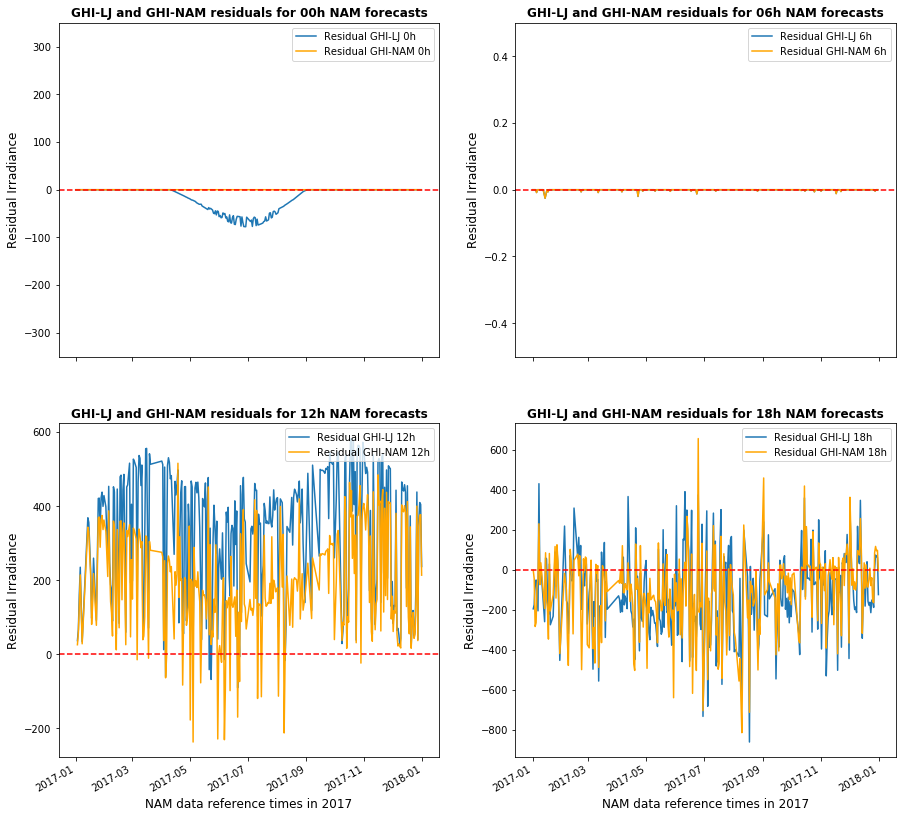
\includegraphics[width=\textwidth]{chapter4/fig_ghi_comparison_lj.png}
    	\caption[Comparing GHI from Liu Jordan Model ($GHI_{LJ}$) and GHI from NAM Forecast Model ($GHI_{NAM}$) for 00h, 06h, 12h, 18h forecasts in 2017]{Comparing GHI from Liu Jordan Model ($GHI_{LJ}$) and GHI from NAM Forecast Model ($GHI_{NAM}$) for 00h, 06h, 12h, 18h forecasts: Residuals of $GHI_{CS}$ and $GHI_{NAM}$ with respect to Array B irradiance observations (left); Clearness index ($K_t$) estimations for individual forecasts in 2017 (right).}
    	\label{fig:fig_ghi_comparison_lj}
    \end{center}
\end{figure}

\par In order to analyze the $GHI$ values from both NAM model and Liu Jordan model, residuals between the irradiance observations from solar array B and both $GHI\textsubscript{NAM}$ and $GHI\textsubscript{LJ}$ were estimated for the year 2017. Among these, the residuals corresponding to the 00h, 06h, 12h and 18h UTC forecasts were separated, and were plotted in Fig.~\ref{fig:fig_ghi_comparison_lj} (left). Clearness index is extremely important in the parameterization of Liu-Jordan model. Thus, it was evaluated for each of the forecasts, and corresponding plots were drawn in Fig.~\ref{fig:fig_ghi_comparison_lj} (right). It was observed that the clearness index too, like clear-sky index in Fig.~\ref{fig:fig_ghi_comparison_lj} was constantly zero for the 06h forecasts throughout the year. This can be attributed to the fact that these forecasts correspond to the time of darkness. However, unlike the clear-sky index metric, which is constantly zero for the 00h forecasts as well, it was observed that the clearness index resulted in a significant non-zero plot for few of the 00h forecasts, indicating that GHI was wrongly estimated for these forecasts, which the clearness metric couldn't ascertain.

\par In the Liu Jordan model, DNI is estimated from transmittance, DHI based on transmittance and solar zenith angle, and GHI is empirically formulated from DHI and DNI. GHI estimated by the Liu Jordan model is blended into the dataset by averaging the GHI estimates for the 18h NAM forecasts, for which $K_t > 0.7$. Furthermore, Liu Jordan model has been shown to be effective in predicting diffuse irradiance on inclined surfaces. This was also verified as the DHI estimated by this model was observed to have a higher correlation with the ground-based solar irradiance observations. Additionally, it was also observed that the GHI observations through this formulation for the year 2017 are highly correlated with DNI. Thus, to avoid multicollinearity amongst the estimators, only DHI estimated by Liu Jordan model was included along with the estimators from the NAM model for the post-processing of solar irradiance using machine learning models.

\subsubchapter{Predictive Modeling Using Clear-Sky Index}

\subchapter{Results and Discussion}
\par In \cite{thesis_zach}, Jones et al used a 24-hour \textit{persistence model} to set a baseline for the more sophisticated machine learning models. In general, persistence models are based on the assumption that conditions remain unchanged between the current time and a future time. The 24-hour persistence models would measure the solar irradiance at a particular time $t$ based on the irradiance value measured at $t-24$. Making use of such a trivial model as a baseline helps in understanding and preparing the data better, by providing a reference for improving the model. Similar 24-hour \textit{persistence models} were used as a baseline in this work as well.

\par Several machine learning algorithms such as least-squares linear regression (LSLR), k-Nearest Neighbors (KNN), Support Vector Regression (SVR), Decision Trees (DT), Random Forests (RF) and Extreme Gradient Boosted Trees (XGBT) were used for the purpose of forecasting. Weather parameter inputs from the NAM data were used as inputs to the machine learning models, and the irradiance observations from the solar arrays A, B and E were used as the target variables. Prediction of target irradiance was done for a forecast horizon of 24 hours, i.e, solar irradiance on each of the arrays was predicted 24 hours into the future, at a one hour temporal resolution. Models were trained on data collected during 2017, and evaluated against data collected during 2018. The performance of the machine learning models were evaluated based on the metrics such as \textit{mean absolute error (MAE)} and $R^2$.  

\par Separate machine learning models were trained for each of the target hour offsets between 1 and 24, and their results were analyzed in two schemes: mean of the evaluations for each forecast hour in the forecast horizon ($Overall$); mean of the evaluations for sets of six forecast hours in the forecast horizon, i.e, $1 - 6$, $7 - 12$, $13 - 18$ and $19 - 24$. Such an analysis helped in realizing the performance of the models specifically for different periods in the day. 

\par In this work, an input selection scheme as described in 3.2 was incorporated towards selecting features for the machine learning models. As a part of this scheme, the key differences between Jones' dataset and the one used in this work, towards training with the machine learning models are as follows: Jones et al hadn't considered the \textit{total cloud cover} parameter in the NAM weather dataset; from among the other surface weather variables used, only air temperature, height at planetary boundary layer and downward shortwave radiation flux were considered; instead of the 36 feature projections for each of the weather variables, select feature projections depending on the target hour offset were chosen; design of the temporal features was different. Based on these differences, the two NAM datasets were used as input to different machine learning models.


\begin{table}[h]
\begin{center}
    \caption{Sample Table 1}
    \begin{tabular}{ c c c c c c c c c}
    	\toprule
    	\textbf{Metric} & \textbf{Horizon} & \textbf{PER} & \textbf{LSLR} & \textbf{SVR} & \textbf{KNN} & \textbf{DT} & \textbf{RF} & \textbf{XGBT}\\
    	\midrule
    	\multirow{3}{4em}{$MAE$} & $1 - 6$ & \_\_ & \_\_ & \_\_ & \_\_ & \_\_ & \_\_ & \_\_\\ &
    	$7 - 12$ & \_\_ & \_\_ & \_\_ & \_\_ & \_\_ & \_\_ & \_\_\\ &
    	$13 - 18$ & \_\_ & \_\_ & \_\_ & \_\_ & \_\_ & \_\_ & \_\_\\ &
    	$19 - 24$ & \_\_ & \_\_ & \_\_ & \_\_ & \_\_ & \_\_ & \_\_\\ &
    	$Overall$ & \_\_ & \_\_ & \_\_ & \_\_ & \_\_ & \_\_ & \_\_\\
    	\midrule
    	\multirow{3}{4em}{$R^2$} & $1 - 6$ & \_\_ & \_\_ & \_\_ & \_\_ & \_\_ & \_\_ & \_\_ \\ &
    	$7 - 12$ & \_\_ & \_\_ & \_\_ & \_\_ & \_\_ & \_\_ & \_\_\\ &
    	$13 - 18$ & \_\_ & \_\_ & \_\_ & \_\_ & \_\_ & \_\_ & \_\_\\ &
    	$19 - 24$ & \_\_ & \_\_ & \_\_ & \_\_ & \_\_ & \_\_ & \_\_\\ &
    	$Overall$ & \_\_ & \_\_ & \_\_ & \_\_ & \_\_ & \_\_ & \_\_\\
    	\bottomrule
    \end{tabular}
\end{center}
\end{table}

\newpage
\chapter{}{Conclusion \& Future Directions}{Conclusion \& Future Directions}

% Print References
\clearpage
\printbibliography[title={%
    \begin{center}
        \normalsize
        \MakeUppercase{\textbf{References}}
    \end{center}}]

% Add 'References' section to Table of Contents
\addcontentsline{chl}{chapter}{~REFERENCES}

\end{document}
